\documentclass[a4paper]{article}

\usepackage{NotesPackage2}
\usepackage{tocbibind}
\usepackage[utf8]{inputenc}  % for Greek writing
\usepackage[greek,english]{babel}  % for Greek writing
\usepackage{lmodern}  % for Greek writing
\usepackage[T1]{fontenc}  % for alternate ddbar
\usepackage{tablefootnote}

\author{Willoughby Seago}
\date{September 23, 2020}
\title{Thermal Physics}

% constants
\newcommand{\boltzmann}{k_\mathrm{B}}
\newcommand{\avagadro}{N_\mathrm{A}}
\newcommand{\gaylussac}{k_\mathrm{GL}}

% specify part of systems/surroundings/universe
\newcommand{\sys}{{\mathrm{sys}}}
\newcommand{\surr}{{\mathrm{surr}}}
\newcommand{\tot}{{\mathrm{tot}}}

% other
\newcommand{\notesVersion}{1.0}
\newcommand{\notesDate}{23/12/2020}
\newcommand{\ddbar}[1]{\text{\dj}{#1}}
\newcommand{\emf}{\mathcal{E}}
\DeclareSIUnit{\atm}{atm}

\makeglossaries
\newacronym{cpt}{CPT}{charge parity time}
\newacronym{npl}{NPL}{national physical laboratory}
\newacronym{cfc}{CFC}{chloroflurocarbon}

\includeonly{}

\begin{document}
    \pagenumbering{roman}  % Number contents pages and glossaries with roman numerals
    \maketitle
    These are my notes for the \textit{thermal physics} course from the University of Edinburg as part of the third year of the theoretical physics degree.
    When I took this course in the 2020/21 academic year it was taught by Professor Graeme Ackland\footnote{\url{https://www.ph.ed.ac.uk/people/graeme-ackland}} and Professor Alexander Morozov\footnote{\url{https://www.ph.ed.ac.uk/people/alexander-morozov}}.
    These notes are based on the lectures delivered as part of this course, the notes provided as part of this course, and the book `Finn's thermal physics'\footnote{Rex, A. \textit{Finn's Thermal Physics}, third edition (CRC Press, Boca Raton, 2017)}.
    The content within is correct to the best of my knowledge but if you find a mistake or just disagree with something or think it could be improved please let me know.
    
    These notes were produced using \LaTeX\footnote{\url{https://www.latex-project.org/}}.
    Graphs where plotted using Matplotlib\footnote{\url{https://matplotlib.org/}}, NumPy\footnote{\url{https://numpy.org/}}, and SciPy\footnote{\url{https://scipy.org/scipylib/}}.
    Diagrams were drawn with tikz\footnote{\url{https://www.ctan.org/pkg/pgf}}.
    
    This is version \notesVersion~of these notes, which is up to date as of \notesDate.
    \begin{flushright}
        Willoughby Seago
        
        s1824487@ed.ac.uk
    \end{flushright}
    \clearpage
    \tableofcontents
    \listoffigures
    \listoftables
    \printglossary[type=\acronymtype, title=Acronyms, style=long]
    \clearpage
    \pagenumbering{arabic}  % Number rest of document with numbers
    \begingroup
    \let\clearpage\relax  % "\begingroup, \let\clearpage\relax, \endgroup" stops automatic pagebreaks after each include
    % \include sections here
    \endgroup
    \section{The Basics of Thermodynamics}
    \subsection{What is Thermodynamics}
    The word thermodynamics comes from the Greek \textgreek{θερμός} (therm\`os), meaning heat, and \textgreek{δύναμις} (dunamis), meaning motive force.
    Thermodynamics is perhaps best described as the study of moving heat.
    Of particular interest is how to convert heat into motion and vice versa.
    
    One of the most important ideas that we can take away form thermodynamics is a sense of time and causality.
    In classical mechanics everything is based off of Newton's second law,
    \[F = m\dv[2]{x}{t}.\]
    If we replace \(t\) with \(-t\), this is a time transformation all that happens is that the coefficient, \(m\), changes to \(-m\):
    \[F = -m\dv[2]{x}{t}.\]
    This is simply a statement that all process in classical mechanics are reversible.
    In electromagnetism everything can be built up from Maxwell's equations.
    Two of these are
    \[\curl\vv{E} = -\partial_t\vv{B},\]
    and
    \[\curl\vv{H} = \vv{J} + \partial_t\vv{D}.\]
    If we replace \(t\) with \(-t\) in the first of these we get
    \[\curl\vv{E} = \partial_t\vv{B},\]
    all that happens is the cross product is negated.
    This is equivalent to changing from a right handed to left handed system, this is a parity transformation.
    If we replace \(t\) with \(-t\) in the second equation and change from a right to left handed system we get
    \[\curl\vv{H} = -\vv{J} + \partial_t\vv{D}.\]
    This is equivalent to setting all charges, \(q\), equal to \(-q\).
    This is a charge transformation.
    In quantum mechanics everything is based upon the Schr\"odinger equation:
    \[\frac{1}{2m}\laplacian\psi + V\psi = i\partial_t\psi\]
    if we replace \(t\) with \(-t\) we get
    \[\frac{1}{2m}\laplacian\psi + V\psi = -i\partial_t\psi\]
    however both \(i\) and \(-i\) have the important property of squaring to \(-1\).
    This means that this time transformation is the same as choosing to take the negative square root instead of the positive.
    
    The important thing about all of these transformations is that if we reverse time \((t \to -t)\), parity \((\text{right}\to\text{left})\), charge \((q\to-q)\), as well as which square root we take none of the physics changes.
    This is called \acrfull{cpt} symmetry and is the only symmetry of C, P, and T that exists.
    CP, CT, and PT symmetry are all violated by some processes in nature but \acrshort{cpt} symmetry isn't.
    This means that all of physics is time reversible if we just reverse a few other things at the same time.
    This is not true for thermodynamics.
    The second law of thermodynamics states that entropy will always increase.
    This means we cannot reverse time.
    This gives us a way to define cause and effect.
    
    \subsection{Equilibrium}
    An \define{equilibrium state} is one in which all bulk physical properties do not change with time and are uniform throughout the system.
    Uniformity only happens if the system is in the same phase throughout.
    If there is a phase boundary then he system can be split into two or more homogeneous portions, one for each phase.
    Within each of these portions the properties are uniform, this is what \define{homogeneous} means.
    
    Isolated systems have equilibrium states that they settle into.
    Equilibrium states have uniform macroscopic properties, such as pressure, temperature, density, and magnetisation.
    Surrounding systems need not be in equilibrium with each other.
    
    \subsection{System}
    The \define{system} is the sample of interest.
    The system interacts with its surroundings.
    The system and its surroundings are separated by some kind of boundary wall.
    The type of boundary wall defines what is held constant, for example
    \begin{enumerate}
        \item if the boundary wall is a moving piston then volume is not held constant.
        A system where volume \emph{is} held constant is called \define{isovolumetric}.
        \item if the wall is well insulated the amount of heat energy is held constant.
        A system where the amount of heat energy is held constant is called \define{adiabatic}.
        \item A system that is not insulated will have temperature held constant.
        A system where temperature is held constant is called \define{isothermic}.
    \end{enumerate}
    In a thermodynamic process the way in which system variables change depends on the surroundings.
    
    \subsection{State Functions/Variables}
    Thermodynamics is about macroscopic properties.
    We care about the temperature, not the speed of individual particles.
    We care about the volume, density, or mass, not the number of particles.
    The various properties that can be quantified without disturbing the system are called \define{state functions} or \define{state properties}.
    For example, the internal energy, volume, pressure, and temperature are state functions.
    Properties whose absolute (as opposed to relative) values are easily measured are called \define{state variables}.
    For example, the volume, pressure, and temperature are state variables but the internal energy is not.
    Relations between state functions are called the \define{equations of state} of the material.
    For example for an ideal gas one equation of state is the ideal gas law:
    \[PV = nRT.\]
    
    \subsection{Zeroth Law of Thermodynamics}
    We define two systems to be in thermal contact if it is possible for heat to move from one to the other.
    We define two systems to be in thermal equilibrium if they could be put in thermal equilibrium without any net heat flow between them.
    The zeroth law of thermodynamics is an experimentally law.
    It states:
    \paragraph{Zeroth Law:} If two systems are in thermal equilibrium with another system then the are in thermal equilibrium with each other.
    
    This can be extended to any number of systems.
    The relation, \(\sim\), defined by \(A\sim B\) if and only if \(A\) is in thermal equilibrium with \(B\) is an equivalence relation and the zeroth law is a statement of the transitivity of \(\sim\).
    
    \subsection{Temperature}
    If systems are in thermal equilibrium with each other they must have some property with a common value.
    We will call this property the thermodynamic temperature, \(T_0\), where the 0 denotes that this value is derived from the zeroth law.
    Note that this is not a numerical system.
    All we can say given two systems is that they are either in thermal equilibrium or they aren't and if they aren't then we define the hotter one to be the one that is losing heat energy.
    
    From the ideal gas equation we have
    \[T_\mathrm{IG} = \frac{PV}{nR}\]
    which gives us another definition of temperature.
    This time \(T_\mathrm{IG}\) is a numeric scale.
    This scale relates to macroscopic properties.
    
    We can also define a third temperature system based off of the kinetic properties of particles:
    \[\frac{1}{2}m\bar{v}^2 = \frac{3}{2}\boltzmann T_\mathrm{K}\]
    \(T_\mathrm{K}\) is again a numerical scale which now relates to the microscopic property of average kinetic energy.
    
    The amazing thing is that it turns out that all three temperature systems, \(T_0\), \(T_\mathrm{IG}\) and \(T_\mathrm{K}\), actually are all equivalent so can be viewed as one temperature system, \(T\), which relates to the zeroth law, the macroscopic properties and the microscopic properties of the system.
    
    The base point for temperature was changed recently.
    We used to use absolute zero and the triple point of water to define two points on the scale and then filled in around that.
    We still use absolute zero, we just use a different upper point.
    It is based off the speed of sound in a gas which is given by
    \begin{equation}\label{eqn:speed of sound in gas}
        c_0 = \sqrt{\pdvconst{P}{\rho}{S}} = \sqrt{\frac{\gamma P}{\rho}}\ = \sqrt{\frac{\gamma\avagadro\boltzmann T}{M}}.
    \end{equation}
    In July 2013 the \acrfull{npl} measured
    \[\boltzmann = \SI{1.38065156(98)e-23}{\joule.\kelvin^{-1}}.\]
    The speed of sound in argon was also measured using a copper sphere whose diameter was known to \(\SI{11.7}{\nano\metre}\), which is approximately 500 atoms in a row.
    The accurate measure of these values allowed for equation~\ref{eqn:speed of sound in gas} to be used to specify a particular temperature more accurately than the triple point of water could.
    For this reason this is now taken as part of the definition of our temperature scale.
    
    \section{Reversibility}
    \subsection{Processes}
    In Thermodynamics a process is the change of a state variable with time.
    If a process is reversible then every (infinitesimal) step is reversible for both the system and the surroundings.
    This involves moving in between equilibrium states.
    A reversible process is quasi-static, meaning that if the external driving force is removed then the process will halt as it is in an equilibrium state.
    
    An irreversible process is the opposite of a reversible process.
    It involves moving away from equilibrium states.
    This means that the state variables are not necessarily the same everywhere during an irreversible process.
    This means that even something as simple as
    \[\int_{P_1}^{P_2}\,\dd{P}\]
    can be undefined if \(P\) is not the same throughout the system.
    
    In general reversible processes involve a slow process such as a slow compression that allows the system to relax to equilibrium between each infinitesimal step.
    The equivalent irreversible process would be pushing the piston in quickly.
    This causes turbulence which is a dissipative process and causes energy to be lost to the surroundings as heat, which is hard to recapture.
    
    When drawing on an indicator diagram, such as a \((P, V)\) diagram, if a process is reversible it can be represented as a continuous line.
    If it is irreversible this may not be possible.
    Instead we draw a series of circles representing the range of values that the state variables take at any one time.
    
    It is possible to move between two states by a reversible or irreversible process.
    The final state of the system will be the same regardless of reversibility.
    However the state of the surroundings will be different for the different processes.
    
    \begin{example}
        Consider a piston of area \(A\) being pushed in a distance, \(\dd{x}\), by a force, \(F\).
        The force required is given by \(F = PA\) which is simply the definition of pressure, \(P\).
        The volume change is \(\dd{V} = A\dd{x}\).
        The work done is \(\dd{W} = F\dd{x} = PA\dd{x} = P\dd{V}\).
        For this reason we define work in thermodynamics as \(\dd{W} = (-)P\dd{V}\).
        If we now wish to find the work done for a finite volume change from \(V_1\) to \(V_2\) we simply integrate:
        \[W = \int_{W_1}^{W_2}\dd{W} = \int_{V_1}^{V_2}P\,\dd{V}.\]
        The total work depends exactly on what the process is.
        If \(P\) is a constant then this integral is trivially \(P(V_2 - V_1)\).
        If we assume an ideal gas then the integral depends on whether we take \(T\) as a constant or try to quantify how it changes.
    \end{example}
    \begin{example}\label{exa:reversible ideal gas expansion}
        Consider an ideal gas that expands reversibly from a state, \((P_1, V_1, T_1)\), to a state, \((P_2, V_2, T_2)\).
        Again the work done is
        \[W = \int_{V_1}^{V_2}P\,\dd{V}.\]
        \begin{figure}[ht]
            \centering
            \begin{tikzpicture}
                \draw[<->] (0, 4) -- (0, 0)-- (4, 0);
                \draw (1, 3) -- (1, 1) -- (3, 1);
                \begin{scope}
                    \clip (1, 1) rectangle (3, 3);
                    \draw (3, 3) circle[radius=2cm];
                \end{scope}
                \draw[dashed] (1, 1) -- (1, 0);
                \draw[dashed] (3, 1) -- (3, 0);
                \draw[dashed] (1, 1) -- (0, 1);
                \draw[dashed] (1, 3) -- (0, 3);
                \node[below] at (1, 0) {\(V_1\)};
                \node[below] at (3, 0) {\(V_2\)};
                \node[left] at (0, 1) {\(P_1\)};
                \node[left] at (0, 3) {\(P_2\)};
                \node[right] at (4, 0) {\(V\)};
                \node[above] at (0, 4) {\(P\)};
                \draw[->] (1, 3) -- (1, 2);
                \draw[->] (1, 1) -- (2, 1);
                \draw[->] (1.59, 1.59) -- (1.591, 1.589);
                \node[left] at (1, 2) {\(A\)};
                \node[below] at (2, 1) {\(B\)};
                \node[above right] at (1.59, 1.59) {\(C\)};
            \end{tikzpicture}
            \caption{Two possible processes for a reversible expansion.}
            \label{fig:reversible ideal gas expansion}
        \end{figure}
        Consider figure~\ref{fig:reversible ideal gas expansion}.
        The path marked \(C\) is an isothermal process.
        This makes it easy to define the pressure using the ideal gas law with \(T = T_1 = T_2\):
        \[P = \frac{nRT}{V}.\]
        Thus the work done becomes
        \begin{align*}
            W &= \int_{V_1}^{V_2}P\,\dd{V}\\
            &= nRT\int_{V_1}^{V_2}\frac{\dd{V}}{V}\\
            &= nRT\ln\left(\frac{V_2}{V_1}\right).
        \end{align*}
        If instead we consider the non-isothermal process along path \(A\) then \(B\) we end up at the same point.
        This time we have to do two integrals.
        The first is along \(A\) and the second along \(B\).
        Thus the work is
        \begin{align*}
            W &= \int_A P\,\dd{V} + \int_B P\,\dd{V}\\
            &= \int_{V_1}^{V_1}P\,\dd{V} + \int_{V_1}^{V_2}P\,\dd{V}\\
            &= 0 + P\int_{V_1}^{V_2}\dd{V}\\
            &= P(V_2 - V_1).
        \end{align*}
        Here we have used the fact that an integral over \([V_1, V_1]\) is zero so we don't need to know the pressure.
        We then used the fact that the process that takes us along \(B\) is isobaric (constant pressure) so we can factor the pressure out of the integral.
        
        We see that we get two different results for the work done depending on the process, even for a reversible process like this one.
        In fact we could do an infinite amount of work by just cycling along path \(A\) then \(B\) and then backwards along \(C\).
    \end{example}
    
    \subsection{Sign Convention}
    In physics and chemistry we are usually interested in changes of the system.
    In engineering the interest is usually in changes of the surroundings.
    For this reason there is a difference in sign conventions used to define work.
    It could be \(\pm P\dd{V}\).
    We choose\footnote{We will explain the bar through the \(\dd\) in a couple of sections}
    \[\ddbar{W} = -P\dd{V}.\]
    The logic behind this is that if \(\dd{V} < 0\), i.e. the system is compressed, then the work done is positive.
    We expect the work done to compress a gas to be positive so this is the correct sign choice for us.
    The important thing is to think about the sign that you expect \emph{before} attempting a problem.
    
    \subsection{Dissipative Processes}
    For an irreversible process we can't specify the work done by the state variables as these aren't well defined.
    We can measure the work done on/by the surroundings and use conservation of energy to say what this means for work done on/by the system.
    
    An example of a dissipative process is stirring.
    The system heats up but \(P\dd{V} = 0\) as the volume doesn't change.
    This means this can't possibly be the correct form of the work done.
    So this process must be dissipating energy in some way.
    If you stir in the opposite direction, i.e. perform the reverse process, it isn't possible to un-mix or extract energy.
    We see that stirring is not a reversible process.
    
    Dissipative processes are always irreversible, however not all irreversible processes are dissipative.
    
    \subsection{The Maths of Thermodynamics}
    In thermodynamics we often ask the questions
    \begin{itemize}
        \item How does changing one state variable affect another -- this points us towards differential calculus as a solution.
        \item How does constraining one variable while changing a second affect a third variable -- this points us to partial derivatives.
    \end{itemize}
    
    \subsubsection{Exact Differentials}
    Consider a single valued state function, \(\varphi\), of the variables \(x\) and \(y\).
    If we change \(x\) by \(\dd{x}\) and \(y\) by \(\dd{y}\) the change in \(\varphi\) is given by
    \[\dd{\varphi} = \pdvconst{\varphi}{x}{y}\dd{x} + \pdvconst{\varphi}{y}{x}\dd{y}.\]
    The same can be done for a function of more variables.
    The finite change in \(\varphi\) is given by
    \[\Delta\varphi = \varphi(x_2, y_2) - \varphi(x_1, y_1) = \int_{(x_1, y_1)}^{(x_2, y_2)} \dd{\varphi}.\]
    So we see that \(\Delta\varphi\) is uniquely determined by its evaluation at the two points \((x_1, y_1)\), and \(x_2, y_2\).
    The integral is path independent.
    State variables in thermodynamics have path independent integrals.
    
    For example if a process takes a system from the state \((T_1, P_1)\) to \((T_2, P_2)\) then we can find another state variable by integrating along any path between these two points.
    So we may as well choose one that makes the integral as easy as possible.
    
    We can calculate the change of a state variable due to an irreversible process by calculating the change of that state variable due to an equivalent reversible process.
    This is only true for the system.
    We can't do this for the surroundings as the state of the surroundings changes depending on if we follow a reversible or irreversible process but by definition the system is in the same state at the beginning and end of the process.
    
    All state variables, \(f\), of the variables \(x_i\) have the property that
    \[\pdvsec{f}{x_i}{x_j} = \pdvsec{f}{x_j}{x_i}\]
    where all the variables that aren't explicitly included are held constant.
    This means that \(f\) is a well behaved, differentiable, function.
    State variables are almost always well behaved, the one exception is at a phase transition, for example the volume can change discontinuously upon boiling.
    
    If we have two independent variables and \(f\) depends on both of them then the variables that we hold constant are important.
    For the following derivatives describe isothermal and isobaric compression and are in general not equal:
    \[\pdvat{f}{V}{T} \ne \pdvat{f}{V}{P}.\]
    
    \subsubsection{Inexact Differentials}
    If something is not a state variable then it does not have an exact differential.
    We denote the inexact differential with a bar, such as \(\ddbar{W}\), to remind us of this.
    The integral over this variable is dependent on the path, this is what it means to be inexact.
    We consider the argument from before in reverse.
    Suppose that the integral over \(\ddbar{\varphi}\) is path dependent.
    Therefore we cannot simply write
    \[\int\ddbar{\varphi} = \varphi(\vv{x}_2) - \varphi(\vv{x}_1)\]
    where \(\vv{x}_1\) and \(\vv{x_2}\) are simply vectors of state variables.
    The fact that we can't write this means that \(\varphi\) is not a state function.
    
    Work is not a state function.
    We can show this by showing that the order of partial derivatives matters.
    The inexact differential for work is \(\ddbar{W} = -P\dd{V}\).
    The question that we ask is if there exists a function, \(W\), of variables \(P\) and \(T\) such that
    \[\dd{W} = \pdvconst{W}{P}{V}\dd{P} + \pdvconst{W}{V}{P}\dd{V}?\]
    We still require that \(\ddbar{W} = -P\dd{V}\) so from this we must have
    \[\pdvconst{W}{P}{V} = 0,\qquad\text{and}\qquad \pdvconst{W}{V}{P} = -P.\]
    Calculating second derivatives we get
    \begin{align*}
        \pdv{V}\left(\pdvconst{W}{P}{V}\right)_{P} &= \pdv{V}\left(0\right)_{P} = 0\\
        \pdv{P}\left(\pdvconst{W}{V}{P}\right)_{V} &= \pdv{P}\left(-P\right)_{V} = -1
    \end{align*}
    Since \(0 \ne -1\) we have that
    \[\pdvsec{W}{P}{V} \ne \pdvsec{W}{V}{P}.\]
    Hence \(W\) is not a state function.
    The order of derivatives is important and the integral is path dependent.
    Remember that in example~\ref{exa:reversible ideal gas expansion} the path that we chose affected the work done.
    
    To summarise
    \begin{itemize}
        \item State variables in thermodynamics have path independent integrals.
        \item Reversible processes in thermodynamics have path dependent integrals.
        \item Irreversible processes in thermodynamics have no well defined integrals.
    \end{itemize}
    
    \begin{example}
        The state of a fluid undergoes an infinitesimal, reversible, change from \((P, T)\) to \((P + \dd{P}, T + \dd{T})\).
        What is the change in volume?
        Start by writing the volume as a function of relevant state variables, \(V = V(P, T)\).
        The change in volume is then
        \begin{align*}
            \dd{V} &= \pdvconst{V}{P}{T}\dd{P} + \pdvconst{V}{T}{P}\dd{T}\\
            &= -\frac{K}{V}\dd{P} + \beta V\dd{T}
        \end{align*}
        where \(K\) is the bulk modulus, which characterises isothermic compression, and \(\beta\) is the thermal expansivity, which characterises isobaric compression.
        They are defined by
        \[K = -V\pdvconst{P}{V}{T},\qquad\text{and}\qquad\beta = \frac{1}{V}\pdvconst{V}{T}{P}.\]
        \(V\) is a state function so we can choose any path.
        We choose a reversible, two-stage path; an isotherm from \(P\) to \(P + \Delta P\) and then an isobar from \(T\) to \(T + \Delta T\).
        The total volume change is then given by the integral over these two paths.
        For the first path \(\dd{T} = 0\) as it is an isotherm.
        Thus we have
        \[\int\frac{1}{V}\,\dd{V} = -\int\frac{1}{K}\,\dd{P} \implies \ln\left(\frac{V_2}{V_1}\right) = -\frac{\Delta P}{K}.\]
        For the second path \(\dd{P} = 0\) as it is an isobar.
        Thus we have
        \[\int\frac{1}{V}\,\dd{V} = -\int\beta\,\dd{T} \implies \ln\left(\frac{V + \Delta V}{V_1}\right) = \beta\Delta T.\]
        After some rearranging we get
        \[V + \Delta V = Ve^{-\Delta P/K}e^{\beta\Delta T}.\]
        Notice that \(V_1\) disappears as this was just an intermediate value that we introduced to define a path.
        We would have also gotten the same result if we started with the isobar and then the isotherm.
        If we had considered an irreversible process the answer would have been the same even though the integral is not defined for that process.
    \end{example}
    
    \section{Heat}
    Take some ice, put it in some water.
    Does all the ice melt?
    What temperature does the water end up?
    The process for answering these questions is to consider the following process:
    \begin{itemize}
        \item The water cools to \(\SI{0}{\degreeCelsius}\).
        This releases \(Q_l = m_lc_l\Delta T_l\) where the symbols have their usual meanings and \(l\) denotes that these are for the liquid water.
        \item The ice warms to \(\SI{0}{\degreeCelsius}\).
        This takes \(Q_s = m_sc_s \Delta T_s\) where \(g\) denotes that these are for the solid water.
        \item The ice melts. This takes \(E = m_s l_\text{vap}\).
        \item Depending on the sign of the left over energy one of two things will happen next:
        \begin{itemize}
            \item If the left over energy is positive it is used to heat the water by \(\Delta T = (Q_l + Q_s + E)/[(m_l + m_s)c_l]\).
            \item If the left over energy is negative some of the ice freezes again.
            We end up with a mass of ice given by \(m = -(Q_1 + Q_s + E)/l_\text{vap}\).
        \end{itemize}
    \end{itemize}
    This successfully answers the question even though this process is not the same as what actually happens.
    For example if the energy left at the end is negative then not all the ice will melt in the first place.
    The fact that we can do this means there must be a state function related to the energies that we are computing with.
    We will see later in this section what that is.
    
    \subsection{What is Heat?}
    James Joule used falling weights to turn paddles in water and measured a temperature rise.
    He found that the same amount of mechanical work, \(mgh\), always produced the same rise in temperature.
    He also found that he could use electrical work to produce this same temperature rise.
    This showed that heat could be produced by work alone.
    Previously heat had been thought of as an element that each material had a finite amount of and could be released by processes such as burning.
    However by putting in an arbitrary amount of mechanical or electrical work Joule showed that an arbitrary amount of heat could be produced and so it necessarily had to come from the work.
    
    As a result of being able to use different forms of work to produce the same change in a system we must have that when a thermally isolated system is brought from one equilibrium state to another the work necessary is independent of the process used.
    This observation requires that there is a state function related to heat, we call it the internal energy, \(U\).
    It was found that
    \[\Delta U = U_2 - U_1 = W_\text{adiabatic}\]
    where the last term is the work done in a process that allows no heat to flow out of the system.
    Essentially this means that the work done in a process, if it can't go anywhere else, goes to increase the internal energy of the system.
    Notice that this equation doesn't give us a way to define a point where \(U = 0\), we can only define internal energy relative to the internal energy in some other state.
    
    This equation is a restricted form of the first law of thermodynamics.
    In this form it applies only to a thermally insulated system and cannot be applied to the whole universe.
    
    If we now allow heat transfer then we find that
    \[\Delta U = U_2 - U_1 = W + Q\]
    where \(W\) is the work done on the system and \(Q\) is the heat going into the system (in other contexts this may have a different sign for heat leaving the system).
    Heat is the exchange of internal energy between the system and the surroundings that cannot be identified as work.
    
    What counts as heat therefore depends on how we define our system.
    If we have a room with a heater and a box of gas then there are two logical ways to define the system.
    The first is as just the box of gas.
    In this case the energy given out by the heater which is absorbed by the gas is counted as heat.
    If instead we define the whole room as the system then the heater is no longer a source of heat for the system it is a source of electrical work and, assuming the walls are well insulated, \(Q = 0\).
    In a way heat and work are just two sides of the same coin.
    
    \subsection{First Law of Thermodynamics}
    \paragraph{First Law:} The change in internal energy, \(\dd{U}\), of a system is given by the sum of the work done on the system, \(\ddbar{W}\), and the heat transferred to the system, \(\ddbar{Q}\):
    \[\dd{U} = \ddbar{W} + \ddbar{Q}.\]
    
    Note that \(\int\ddbar{W}\) and \(\int\ddbar{Q}\) are both path dependent but their sum, \(\int\dd{U}\) is not.
    Often we are interested in the work done mechanically on a compressible fluid\footnote{Remember that fluid encompasses both liquids and gasses.}, we know in this case that the work done is \(\ddbar{W} = -P\dd{V}\) and so the first law of thermodynamics is
    \[\dd{U} = -P\dd{V} + \ddbar{Q}.\]
    
    Typical forms of work that we need to account for are electrical, magnetic, or gravitational.
    Typical forms of internal energy are kinetic energy and potential energy, which in turn includes chemical, nuclear, and gravitational energy, as well as mass energy due to relativity.
    Fortunately since internal energy is always defined relatively we only need to account for sources of internal energy that change.
    For example if we are compressing a gas we don't need to account for chemical, nuclear, gravitational, or mass energy unless we start compressing the gas so much that it starts reacting with itself or undergoing nuclear fusion, and this is unlikely.
    
    Another important feature is that due to the path independence of \(\int\dd{U}\) the first law of thermodynamics has time reversal symmetry.
    
    \subsection{Heat Capacity}
    The heat capacity, \(C\), of a material that is heated by \(\Delta Q\), and has a temperature increase of \(\Delta T\). is defined to be
    \[C = \lim_{\Delta T\to 0} \frac{\Delta Q}{\Delta T} = \dv{Q}{T}.\]
    This definition is useful for theoretical work but for practical calculations we define two more useful quantities: the specific heat capacity, \(c = C/m\),  where \(m\) is the mass of the system, the specific heat capacity then gives the energy needed to heat \(\SI{1}{\kilogram}\) of the substance by \(\SI{1}{\kelvin}\).
    We also define the molar heat capacity, \(c = C/n\)\footnote{Yes, that is the same symbol as specific heat capacity, thermodynamics has too many letters, and an inexplicable refusal to use Greek letters like any other self respecting field of physics would.}, where \(n\) is the number of moles of the substance, the molar heat capacity then gives the energy needed to heat \(\SI{1}{\mole}\) of the substance by \(\SI{1}{\kelvin}\).
    
    As normal with thermodynamics a definition that doesn't specify what is constant isn't very useful.
    If we hold volume constant then the heat capacity at constant volume is \(C_V\).
    We start with a rearrange form of the first law of thermodynamics:
    \[\dd{Q_V} = \dd{U_V} + P\dd{V_V}.\]
    Importantly we are holding \(V\) constant so \(\dd{V_V} = 0\) which means \(\dd{Q_V} = \dd{U_V}\).
    \[C_V = \pdvconst{Q}{T}{V} = \pdvconst{U}{T}{V}.\]
    If instead we hold the pressure constant then \(\dd{Q_P} = \dd{U_P} + P\dd{V_P}\).
    We define the enthalpy, \(H\), to be \(H = U + PV\).
    In differential form this becomes
    \[\dd{H} = \dd{(U + PV)} = \dd{U} + P\dd{V} + V\dd{P}.\]
    Holding \(P\) constant gives us
    \[\dd{H_P} = \dd{U_P} + P\dd{V_P}\]
    since \(\dd{P_P} = 0\) when pressure is held constant.
    Further we know that \(\dd{U_P} = -P\dd{V_P} + \dd{Q_P}\) so substituting this into the enthalpy gives us
    \[\dd{H_P} = -P\dd{V_P} + \dd{Q_P} + P\dd{V_P} = \dd{Q_P}.\]
    Finally this allows us to calculate the heat capacity at constant pressure:
    \[C_P = \pdvconst{Q}{T}{P} = \pdvconst{H}{T}{P}.\]
    Notice that heat capacity is a state variable, unlike heat.
    
    \subsubsection{Relation Between \texorpdfstring{\(C_V\)}{CV} and \texorpdfstring{\(C_P\)}{CP}}
    From the first law of thermodynamics
    \[\dd{Q_P} = \dd{U_P} P\dd{V_P}\]
    dividing through by \(\dd{T}\) and taking a limiting process while holding pressure constant gives us the heat capacity at constant pressure again:
    \begin{equation}\label{eqn:C_P}
        C_P = \pdvconst{Q}{T}{P} = \pdvconst{U}{T}{P} + P\pdvconst{V}{T}{P}
    \end{equation}
    Now let \(U = U(T, V)\), then a small change in these state variables produces the following change in \(U\):
    \begin{equation}\label{eqn:dU}
        \dd{U} = \pdvconst{U}{T}{V}\dd{T} + \pdvconst{U}{V}{T}\dd{V}
    \end{equation}
    Dividing through by \(\dd{T}\) and taking a limiting process while holding pressure constant gives us
    \[\pdvconst{U}{T}{P} = \pdvconst{U}{T}{V} + \pdvconst{U}{V}{T}\pdvconst{V}{T}{P}.\]
    We can identify the first term on the right hand side as \(C_V\):
    \[\pdvconst{U}{T}{P} = C_V + \pdvconst{U}{V}{T}\pdvconst{V}{T}{P}.\]
    We can now substitute this into equation~\ref{eqn:C_P} to get
    \[C_P = C_V + \pdvconst{U}{V}{T}\pdvconst{V}{T}{P} + P\pdvconst{V}{T}{P}.\]
    Subtracting \(C_V\) and factorising we get
    \[C_P - C_V = \left[P + \pdvconst{U}{V}{T}\right]\pdvconst{V}{T}{P}.\]
    This is the best we can do in general, however if we consider an ideal gas then the internal energy is dependent only on the pressure.
    This means that
    \[\pdvconst{U}{V}{T} = 0\]
    for an ideal gas.
    This means
    \[C_P - C_V = P\pdvconst{V}{T}{P}.\]
    From the ideal gas law we have
    \[V = \frac{nRT}{P} \implies \pdvconst{V}{T}{P} = \frac{nR}{P}.\]
    Thus
    \begin{equation}\label{eqn:C_P - C_V = nR ideal gas}
        C_P - C_V = P\frac{nR}{P} = nR.
    \end{equation}
    Now looking at equation~\ref{eqn:dU} for an ideal gas we see that final term is zero and so
    \begin{equation}\label{eqn:dU = C_VdT ideal gas}
        \dd{U} = \pdvconst{U}{T}{V}\dd{T} = C_V\dd{T}.
   \end{equation} 
    We will use this in future calculations.
    
    \subsubsection{Reversible, Isothermal, Ideal Gas Expansion}
    For an isothermal expansion \(\Delta T = 0\).
    The ideal gas law gives us
    \[P = \frac{nRT}{V} \propto \frac{1}{V}\]
    this means that on a \((P, V)\)-indicator diagram we expect isotherms, that is lines of constant temperature, to be hyperbola.
    Since we are considering a reversible process we know that the work done on the system is the negative of the work done on the surroundings.
    We can fairly easily find the work done on the surroundings:
    \[W = \int\ddbar{W} = \int P\dd{V_T} = nRT\int\frac{\dd{V}}{V} = nRT\ln\left(\frac{V_2}{V_1}\right).\]
    
    \subsubsection{Reversible, Adiabatic, Ideal Gas Expansion}
    For an adiabatic expansion \(\Delta Q = 0\) so \(\Delta U = \Delta W\).
    Similarly \(\ddbar{Q} = 0\) so applying equation~\ref{eqn:dU = C_VdT ideal gas} and the first law of thermodynamics gives us
    \[0 = \ddbar{Q} = \dd{U} + P\dd{V} = C_V\dd{T} + P\dd{V}.\]
    Using the ideal gas law to replace \(P\), and then the relationship that we derived for an ideal gas in equation~\ref{eqn:C_P - C_V = nR ideal gas}, that \(C_P - C_V = nR\), we get
    \[0 = C_V\dd{T} + \frac{nRT}{V}\dd{V} = C_V\dd{T} + (C_P - C_V)\frac{T}{V}\dd{V}.\]
    Rearranging gives us
    \[-\frac{C_V}{T}\dd{T} = (C_P - C_V)\frac{1}{V}\dd{V}.\]
    Integrating gives us
    \[-C_V\int\frac{\dd{T}}{T} = (C_P - C_V)\int\frac{\dd{V}}{V}\]
    which we evaluate as
    \[-C_V\ln T = (C_P - C_V)\ln V + \ln A\]
    where \(\ln A\) is a constant of integration.
    Applying log laws gives us
    \[\ln T^{-C_V} = \ln \left(AV^{C_P - C_V}\right).\]
    Exponentiating gives
    \[T^{-C_V} = AV^{C_P - C_V}.\]
    Multiplying through by \(T^{C_V}\) gives
    \[1 = AT^{C_V}V^{C_P - C_V}.\]
    Raising everything to the power of \(1/C_V\) gives
    \[1 = A^{1/C_V}TV^{C_P - 1}.\]
    Multiplying through by \(A^{-1/C_V}\) and defining \(\gamma = C_P/C_V\) we get
    \[A^{-1/C_V} = TV^{\gamma - 1}.\]
    Since \(A\) and \(C_V\) are constants we conclude that \(TV^{\gamma - 1}\) is a constant.
    From the ideal gas law we know that
    \[T = \frac{PV}{nR}\]
    and so the constant \(TV^{\gamma - 1}\) in this form is
    \[TV^{\gamma - 1} = \frac{PV}{nR}V^{\gamma - 1} = \frac{P}{nR}V^\gamma.\]
    Since \(n\) and \(R\) are constants and the left hand side is a constant we must have that \(PV^\gamma\) is constant.
    If instead we write the volume using the ideal gas law:
    \[V = \frac{nRT}{P}\]
    then the constant \(PV^\gamma\) becomes
    \[PV^\gamma = P\left(\frac{nRT}{P}\right)^\gamma = P^{1 - \gamma}(nR)^\gamma T^\gamma.\]
    Since \(\gamma\) is a constant and so are \(n\) and \(R\) we have that \(P^{1-\gamma}T^\gamma\) is a constant, or as it is more usually written by raising everything to the power of \(1/\gamma\): \(TP^{(1 - \gamma)/\gamma}\) is constant.
    
    \subsection{Irreversible Free Expansion and the Joule Coefficient}\label{sec:irreversible free expansion and the Joule coefficient}
    A rigid, adiabatic, container is partitioned into two equal volumes, one which is a vacuum and the other which contains a gas.
    The system we consider is this all of the gas in the container.
    The irreversible process in question is the breaking of the partition.
    No work is done on the system and there is no heat transfer so the internal energy is constant and \(\dd{U} = 0\).
    We can write the temperature as a state function, \(T = T(U, V)\).
    A small change in these state variables causes the following change in the temperature:
    \begin{align*}
        \dd{T} &= \pdvconst{T}{V}{U}\dd{V} + \pdvconst{T}{U}{V}\dd{U}\\
        &= \pdvconst{T}{V}{U}\dd{V}\\
        &= \mu_J\dd{V}.
    \end{align*}
    This is the definition of \(\mu_J\), called the \define{Joule coefficient}, it characterises temperature change due to a volume change.
    For an ideal gas \(U\) depends only on the temperature.
    This means that for \(U\) to be constant we must have the state start and end at the same temperature.
    Therefore \(\mu_J = 0\).
    
    \section{Heat Engines}
    A heat engine turns heat into work.
    They do so by a cyclic process.
    Every cycle the system returns to an initial equilibrium.
    However the surroundings do not return to the same state and work is done.
    All of the steps of the cycle are quasi-static meaning reversible.
    During each step the values of the state variables change and the system exchanges heat and mechanical energy with its surroundings.
    
    \subsection{Carnot Engine}
    The most efficient heat engine is the Carnot engine.
    It follows that Carnot cycle:
    \begin{itemize}
        \item Isothermal expansion
        \item Adiabatic expansion
        \item Isothermal compression
        \item Adiabatic compression
    \end{itemize}
    During the isothermal expansion heat, \(Q_1\), is absorbed, then during the isothermal compression heat, \(Q_2\), is given out.
    The stages drawn on a \((P, V)\)-indicator diagram form a closed loop.
    The work done is the area enclosed by this loop.
    The surroundings of the Carnot engine consist of two constant temperature heat reservoirs.
    In each step of the process there is a piston moving.
    The heat exchange can only occur along the isotherms since by definition there is no heat exchange along an adiabat.
    Every cycle the work done is \(W = Q_1 - Q_2\).
    Reversing the process requires an input of work and heat is moved from one reservoir to the other.
    This is the process by which a refrigerator works.
    \subsection{General Heat Engine}
    \begin{figure}
        \centering
        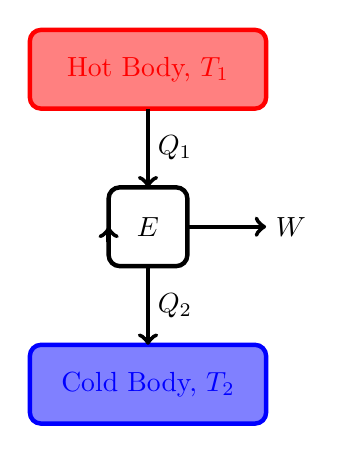
\begin{tikzpicture}
            \tikzstyle{hot} = [color=red, ultra thick, fill=red!50!white, rounded corners]
            \tikzstyle{cold} = [color=blue, ultra thick, fill=blue!50!white, rounded corners]
            \tikzstyle{engine} = [ultra thick, rounded corners]
            \draw[hot] (0, 4) rectangle (3, 5);
            \draw[cold] (0, 0) rectangle (3, 1);
            \draw[engine] (1, 2) rectangle (2, 3);
            \draw[engine, ->] (1, 2.3) -- (1, 2.5);
            \node at (1.5, 2.5) {\(E\)};
            \node[cold] at (1.5, 0.5) {Cold Body, \(T_2\)};
            \node[hot] at (1.5, 4.5) {Hot Body, \(T_1\)};
            \draw[engine, ->] (1.5, 4) -- (1.5, 3);
            \draw[engine, ->] (1.5, 2) -- (1.5, 1);
            \draw[engine, ->] (2, 2.5) -- (3, 2.5);
            \node[right] at (1.5, 3.5) {\(Q_1\)};
            \node[right] at (1.5, 1.5) {\(Q_2\)};
            \node[right] at (3, 2.5) {\(W\)};
        \end{tikzpicture}
        \caption{The basic workings of a heat engine}
        \label{fig:heat engine}
    \end{figure}
    The internal energy is constant.
    Therefore by the first law of thermodynamics we know that
    \[0 = \Delta Q + \Delta W = Q_1 - Q_2 - W \implies W = Q_1 - Q_2.\]
    Notice that we define work done by the engine to be positive as opposed to the more normal work done on the system being positive.
    This is because an engine doing positive work makes more sense so we switch convention when talking about engines.
    The \define{efficiency} of any process is the ratio of useful energy out to total energy in.
    For the heat engine the efficiency is
    \[\eta = \frac{W}{Q_1} = \frac{Q_1 - Q_2}{Q_1} = 1 - \frac{Q_2}{Q_1}.\]
    Perhaps a more useful quantity in practice is the power.
    Power is simply the useful energy per second which is the work done per cycle times the number of cycles per second.
    There is a balance to be had here, we could have very efficient but slow cycles if we were going for peak efficiency but if we want peak power then there will be some optimal speed which may not be at peak efficiency.
    
    \subsection{Second Law of Thermodynamics}
    The second law of thermodynamics defines certain processes to be impossible even if they still follow the first law.
    There are two equivalent statements:
    
    \begin{tabular}{p{0.5\textwidth}p{0.5\textwidth}}
        Clausius statement:
        \paragraph{Second Law:} It is impossible to construct a device that, operating in a cycle, produces no effect other than the transfer of heat from a colder to a hotter body. &
        
        Kelvin--Planck statement:
        \paragraph{Second Law:} It is impossible to construct a device that, operating in a cycle, produces no effect other than the extraction of heat from a single body at a uniform temperature and the performance of an equivalent amount of work.
    \end{tabular}
    Clausius' statement forbids heat to flow from cold to hot even if the total energy is conserved.
    What this means is that for a refrigerator it is impossible to have \(Q_1 = Q_2\) without also putting in work.
    The Kelvin--Planck statement for bids heat to be converted into work with \SI{100}{\percent} efficiency.
    What this means is that for an engine it is impossible to have \(Q_2 = 0\).
    
    Broadly the first law forbids processes where the energy out is different than the energy in and the second law says that the energy out will always have a contribution that we cannot use for driving another process.
    
    We can draw heat engines for the forbidden processes described in both of these statements.
    This is done in figure~\ref{fig:illegal heat engines}
    \begin{figure}[ht]
        \centering
        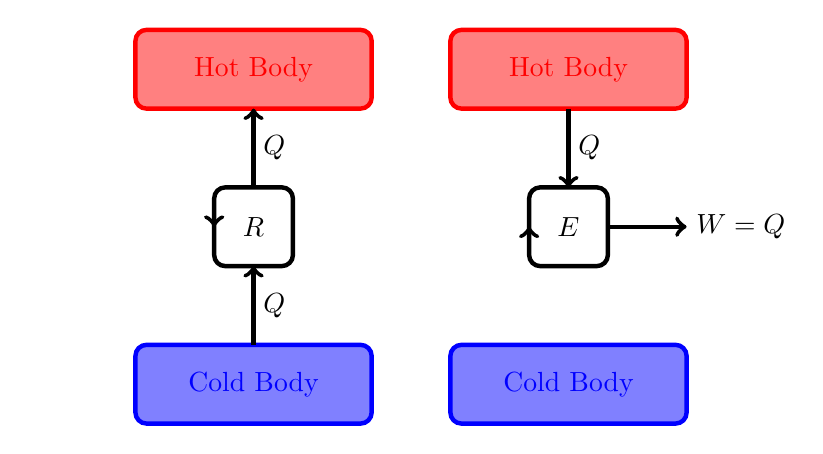
\begin{tikzpicture}
            \tikzstyle{hot} = [color=red, ultra thick, fill=red!50!white, rounded corners]
            \tikzstyle{cold} = [color=blue, ultra thick, fill=blue!50!white, rounded corners]
            \tikzstyle{engine} = [ultra thick, rounded corners]
            
            \draw[hot] (0, 4) rectangle (3, 5);
            \draw[cold] (0, 0) rectangle (3, 1);
            \draw[engine] (1, 2) rectangle (2, 3);
            \draw[engine, ->] (1, 2.7) -- (1, 2.5);
            \node at (1.5, 2.5) {\(R\)};
            \node[cold] at (1.5, 0.5) {Cold Body};
            \node[hot] at (1.5, 4.5) {Hot Body};
            \draw[engine, <-] (1.5, 4) -- (1.5, 3);
            \draw[engine, <-] (1.5, 2) -- (1.5, 1);
            \node[right] at (1.5, 3.5) {\(Q\)};
            \node[right] at (1.5, 1.5) {\(Q\)};
            
            \begin{scope}[xshift=4cm]
                \draw[hot] (0, 4) rectangle (3, 5);
                \draw[cold] (0, 0) rectangle (3, 1);
                \draw[engine] (1, 2) rectangle (2, 3);
                \draw[engine, ->] (1, 2.3) -- (1, 2.5);
                \node at (1.5, 2.5) {\(E\)};
                \node[cold] at (1.5, 0.5) {Cold Body};
                \node[hot] at (1.5, 4.5) {Hot Body};
                \draw[engine, ->] (1.5, 4) -- (1.5, 3);
                \draw[engine, ->] (2, 2.5) -- (3, 2.5);
                \node[right] at (1.5, 3.5) {\(Q\)};
                \node[right] at (3, 2.5) {\(W = Q\)};
            \end{scope}
            \node[color=white, left] at (0, 2.5) {\(W=Q\)};
        \end{tikzpicture}
        \caption{Heat engines forbidden by the second law}
        \label{fig:illegal heat engines}
    \end{figure}
    We can fairly easily show that the two statements of the second law are equivalent.
    First suppose that Kelvin--Planck is false but Clausius still stands.
    We use a Kelvin--Planck violating engine, \(E\), to drive a refrigerator, \(R\).
    If both \(E\) and \(R\) have the same hot and cold bodies then \(E\) extracts heat, \(Q_1\), from the hot body and converts it entirely to work, \(W\), which is then used to run \(R\).
    \(R\) extracts heat \(Q_2\) from the cold body and delivers \(Q_2 + W = Q_2 + Q_1\) to the hot body since the total energy into \(R\) must be equal to the total energy out by the first law.
    If we then treat the system including both \(E\) and \(R\) as one composite refrigerator, \(E + R\), then \(E + R\) extracts \(Q_2\) from the hot body and delivers \(Q_2\) to the cold body.
    This violates Clausius so our assumption that Kelvin--Planck doesn't hold must be wrong.
    Hence Clausius implies Kelvin--Planck.
    We can see the systems in question in figure~\ref{fig:clausius implies kelvin-planck}.
    \begin{figure}[ht]
        \centering
        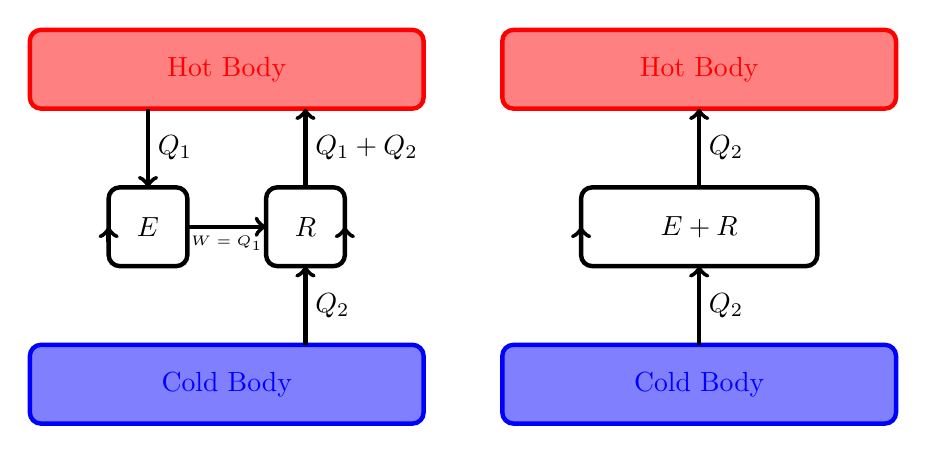
\begin{tikzpicture}
            \tikzstyle{hot} = [color=red, ultra thick, fill=red!50!white, rounded corners]
            \tikzstyle{cold} = [color=blue, ultra thick, fill=blue!50!white, rounded corners]
            \tikzstyle{engine} = [ultra thick, rounded corners]
            \draw[hot] (0, 4) rectangle (5, 5);
            \draw[cold] (0, 0) rectangle (5, 1);
            \draw[engine] (1, 2) rectangle (2, 3);
            \draw[engine, ->] (1, 2.3) -- (1, 2.5);
            \node at (1.5, 2.5) {\(E\)};
            \node[cold] at (2.5, 0.5) {Cold Body};
            \node[hot] at (2.5, 4.5) {Hot Body};
            \draw[engine, ->] (1.5, 4) -- (1.5, 3);
            \draw[engine, ->] (2, 2.5) -- (3, 2.5);
            \node[right] at (1.5, 3.5) {\(Q_1\)};
            \node[below] at (2.5, 2.5) {\tiny\(W = Q_1\)};
            
            \draw[engine] (3, 2) rectangle (4, 3);
            \draw[engine, ->] (4, 2.3) -- (4, 2.5);
            \draw[engine, ->] (3.5, 3) -- (3.5, 4);
            \draw[engine, ->] (3.5, 1) -- (3.5, 2);
            \node[right] at (3.5, 3.5) {\(Q_1 + Q_2\)};
            \node[right] at (3.5, 1.5) {\(Q_2\)};
            \node at (3.5, 2.5) {\(R\)};
            
            \begin{scope}[xshift=6cm]
                \draw[hot] (0, 4) rectangle (5, 5);
                \draw[cold] (0, 0) rectangle (5, 1);
                \draw[engine] (1, 2) rectangle (4, 3);
                \draw[engine, ->] (1, 2.3) -- (1, 2.5);
                \node at (2.5, 2.5) {\(E + R\)};
                \node[cold] at (2.5, 0.5) {Cold Body};
                \node[hot] at (2.5, 4.5) {Hot Body};
                \draw[engine, ->] (2.5, 3) -- (2.5, 4);
                \draw[engine, ->] (2.5, 1) -- (2.5, 2);
                \node[right] at (2.5, 3.5) {\(Q_2\)};
                \node[right] at (2.5, 1.5) {\(Q_2\)};
            \end{scope}
        \end{tikzpicture}
        \caption{A composite system which violates Clausius.}
        \label{fig:clausius implies kelvin-planck}
    \end{figure}
    We can show that Kelvin--Planck implies Clausius in a similar way.
    
    \subsection{Carnot Engine Again}
    Carnot's theorem is
    \paragraph{Carnot's Theorem:} No engine operating between two reservoirs can be more efficient than a Carnot engine operating between the same two reservoirs.
    
    This is fairly easy to prove.
    Suppose that we had an engine \(E'\) with efficiency \(\eta'\) and a Carnot engine \(C\) with efficiency \(\eta_C\).
    Now suppose that \(E'\) violates Carnot's theorem so that when operating between the same reservoirs \(\eta' > \eta_C\).
    We can tune both engines such that they do equal amounts of work, \(W = W'\).
    The efficiency of \(E'\) is
    \[\eta' = \frac{W'}{Q_1'} = \frac{W}{Q_1'}.\]
    The efficiency of \(C\) is
    \[\eta_C = \frac{W}{Q_1}.\]
    For \(\eta' > \eta_C\) to hold we require that
    \[Q_1 > Q_1'.\]
    Since a Carnot engine only exchanges heat along isotherms it is reversible with the same efficiency.
    Thus if we instead use \(C\) as a refrigerator it will have efficiency \(\eta_C\) still.
    If we use \(E'\) to drive \(C\) as a refrigerator then the process acts to move heat \(Q_1 - Q_1'\) from cold to hot without any external work being done.
    Since \(Q_1 > Q_1'\) this quantity is positive so this composite system, \(E' + C\), violates Clausius' statement of the second law.
    This means that our assumption that \(E'\) is more efficient than a Carnot engine is false.
    
    It is however possible that \(\eta' = \eta_C\), this would mean that there is no heat flow in the composite system.
    We conclude that
    \[\eta' \le \eta_C.\]
    \begin{figure}[ht]
        \centering
        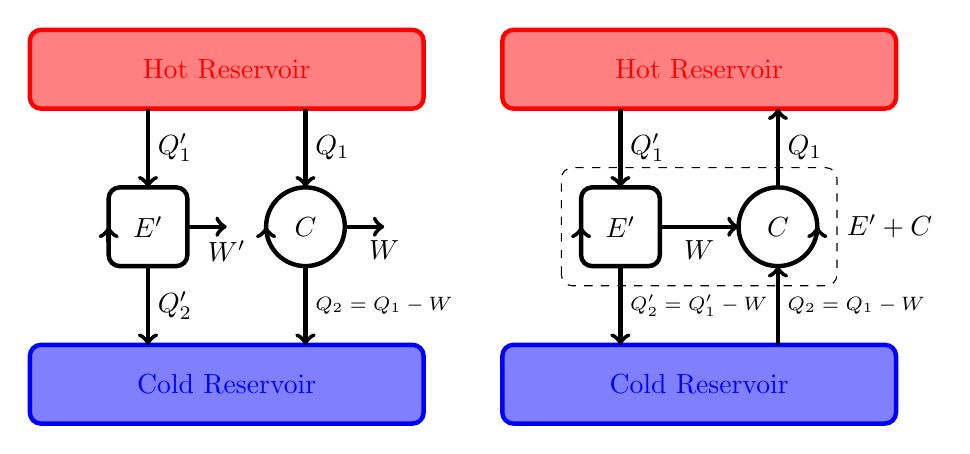
\begin{tikzpicture}
            \tikzstyle{hot} = [color=red, ultra thick, fill=red!50!white, rounded corners]
            \tikzstyle{cold} = [color=blue, ultra thick, fill=blue!50!white, rounded corners]
            \tikzstyle{engine} = [ultra thick, rounded corners]
            \draw[hot] (0, 4) rectangle (5, 5);
            \draw[cold] (0, 0) rectangle (5, 1);
            \draw[engine] (1, 2) rectangle (2, 3);
            \draw[engine, ->] (1, 2.3) -- (1, 2.5);
            \node at (1.5, 2.5) {\(E'\)};
            \node[cold] at (2.5, 0.5) {Cold Reservoir};
            \node[hot] at (2.5, 4.5) {Hot Reservoir};
            \draw[engine, ->] (1.5, 4) -- (1.5, 3);
            \draw[engine, ->] (1.5, 2) -- (1.5, 1);
            \draw[engine, ->] (2, 2.5) -- (2.5, 2.5);
            \node[right] at (1.5, 3.5) {\(Q_1'\)};
            \node[below] at (2.5, 2.45) {\(W'\)};
            \node[right] at (1.5, 1.5) {\(Q_2'\)};
            
            \draw[engine] (3.5, 2.5) circle[radius=0.5cm];
            \draw[engine, ->] (3, 2.49) -- (3, 2.5);
            \draw[engine, <-] (3.5, 3) -- (3.5, 4);
            \draw[engine, <-] (3.5, 1) -- (3.5, 2);
            \draw[engine, ->] (4, 2.5) -- (4.5, 2.5);
            \node[right] at (3.5, 3.5) {\(Q_1\)};
            \node[right] at (3.5, 1.5) {\scriptsize\(Q_2 = Q_1 - W\)};
            \node[below] at (4.5, 2.45) {\(W\)};
            \node at (3.5, 2.5) {\(C\)};
            
            \begin{scope}[xshift=6cm]
                \draw[hot] (0, 4) rectangle (5, 5);
                \draw[cold] (0, 0) rectangle (5, 1);
                \draw[engine] (1, 2) rectangle (2, 3);
                \draw[engine, ->] (1, 2.3) -- (1, 2.5);
                \node at (1.5, 2.5) {\(E'\)};
                \node[cold] at (2.5, 0.5) {Cold Reservoir};
                \node[hot] at (2.5, 4.5) {Hot Reservoir};
                \draw[engine, ->] (1.5, 4) -- (1.5, 3);
                \draw[engine, ->] (1.5, 2) -- (1.5, 1);
                \draw[engine, ->] (2, 2.5) -- (3, 2.5);
                \node[right] at (1.5, 3.5) {\(Q_1'\)};
                \node[below] at (2.5, 2.45) {\(W\)};
                \node[right] at (1.5, 1.5) {\scriptsize\(Q_2' = Q_1' - W\)};
                
                \draw[engine] (3.5, 2.5) circle[radius=0.5cm];
                \draw[engine, ->] (4, 2.49) -- (4, 2.5);
                \draw[engine, ->] (3.5, 3) -- (3.5, 4);
                \draw[engine, ->] (3.5, 1) -- (3.5, 2);
                \node[right] at (3.5, 3.5) {\(Q_1\)};
                \node[right] at (3.5, 1.5) {\scriptsize\(Q_2 = Q_1 - W\)};
                \node at (3.5, 2.5) {\(C\)};
                \draw[dashed, rounded corners] (0.75, 1.75) rectangle (4.25, 3.25);
                \node[right] at (4.25, 2.5) {\(E' + C\)};
            \end{scope}
        \end{tikzpicture}
        \caption{Systems used to prove Carnot's theorem}
    \end{figure}
    
    Suppose that we have two Carnot engines, \(C_a\) and \(C_b\) with efficiencies \(\eta_{C_a}\) and \(\eta_{C_b}\) respectively.
    Since we can use the first to drive the second or vice versa then applying the above proof to these two engines we have \(\eta_{C_a}\le \eta_{c_b}\) and \(\eta_{C_b}\le\eta_{C_a}\) so \(\eta_{C_a} = \eta_{C_b}\).
    This means that all Carnot engines operating between the same two reservoirs have exactly the same efficiency independent of the way that the two engines operate, as long as they follow the Carnot cycle.
    This is a direct Corollary of Carnot's theorem.
    
    Another corollary of Carnot's theorem is a temperature scale.
    Since the efficiency of any reversible heat engine operating between the same two reservoirs is equal the efficiency,
    \[\eta_R = 1 - \frac{Q_2}{Q_1},\]
    can only depend on the temperatures of the reservoirs as these are the only variables that need to be the same for all engines.
    Therefore there must be a universal function, \(f\colon\reals^2 \to \reals\) such that
    \[\frac{Q_2}{Q_1} = f(T_1, T_2)\]
    for all heat engines.
    Here \(T_1\) and \(T_2\) are the temperatures of the hot and cold reservoirs respectively.
    We can consider the form of \(f\) by considering another composite system where one engine runs on the wast heat of another.
    This system is shown in figure~\ref{fig:heat engine running on the heat from a heat engine}.
    Tuning the engines so that \(Q_2 = Q_2'\) we can consider this composite system as a single engine since no net heat enters the reservoir at \(T_3\) so we don't need a reservoir at all.
    \begin{figure}[ht]
        \centering
        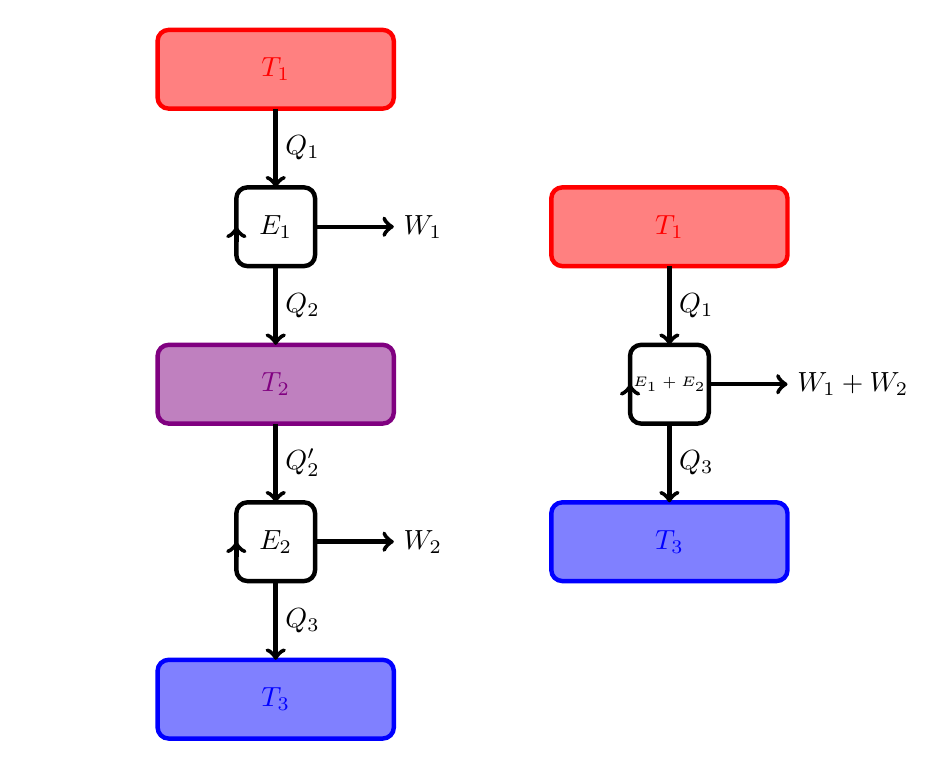
\begin{tikzpicture}
            \tikzstyle{hot} = [color=red, ultra thick, fill=red!50!white, rounded corners]
            \tikzstyle{cold} = [color=blue, ultra thick, fill=blue!50!white, rounded corners]
            \tikzstyle{medium temp} = [color=blue!50!red, ultra thick, fill=blue!50!red!50!white, rounded corners]
            \tikzstyle{engine} = [ultra thick, rounded corners]
            \draw[hot] (0, 4) rectangle (3, 5);
            \draw[medium temp] (0, 0) rectangle (3, 1);
            \draw[cold] (0, -4) rectangle (3, -3);
            \draw[engine] (1, 2) rectangle (2, 3);
            \draw[engine, ->] (1, 2.3) -- (1, 2.5);
            \node at (1.5, 2.5) {\(E_1\)};
            \node[medium temp] at (1.5, 0.5) {\(T_2\)};
            \node[hot] at (1.5, 4.5) {\(T_1\)};
            \node[cold] at (1.5, -3.5) {\(T_3\)};
            \draw[engine, ->] (1.5, 4) -- (1.5, 3);
            \draw[engine, ->] (1.5, 2) -- (1.5, 1);
            \draw[engine, ->] (2, 2.5) -- (3, 2.5);
            \node[right] at (1.5, 3.5) {\(Q_1\)};
            \node[right] at (1.5, 1.5) {\(Q_2\)};
            \node[right] at (3, 2.5) {\(W_1\)};
            \node[color=white, left] at (0, 0.5) {\(W_1 + W_2\)};
            \begin{scope}[yshift=-4cm]
                \draw[engine] (1, 2) rectangle (2, 3);
                \draw[engine, ->] (1, 2.3) -- (1, 2.5);
                \node at (1.5, 2.5) {\(E_2\)};
                \draw[engine, ->] (1.5, 4) -- (1.5, 3);
                \draw[engine, ->] (1.5, 2) -- (1.5, 1);
                \draw[engine, ->] (2, 2.5) -- (3, 2.5);
                \node[right] at (1.5, 3.5) {\(Q_2'\)};
                \node[right] at (1.5, 1.5) {\(Q_3\)};
                \node[right] at (3, 2.5) {\(W_2\)};
            \end{scope}
            \begin{scope}[xshift=5cm, yshift=-2cm]
                \draw[hot] (0, 4) rectangle (3, 5);
                \draw[cold] (0, 0) rectangle (3, 1);
                \draw[engine] (1, 2) rectangle (2, 3);
                \draw[engine, ->] (1, 2.3) -- (1, 2.5);
                \node at (1.5, 2.5) {\tiny\(E_1 + E_2\)};
                \node[hot] at (1.5, 4.5) {\(T_1\)};
                \node[cold] at (1.5, 0.5) {\(T_3\)};
                \draw[engine, ->] (1.5, 4) -- (1.5, 3);
                \draw[engine, ->] (1.5, 2) -- (1.5, 1);
                \draw[engine, ->] (2, 2.5) -- (3, 2.5);
                \node[right] at (1.5, 3.5) {\(Q_1\)};
                \node[right] at (1.5, 1.5) {\(Q_3\)};
                \node[right] at (3, 2.5) {\(W_1 + W_2\)};
            \end{scope}
        \end{tikzpicture}
        \caption{One heat engine running on the waste heat of another.}
        \label{fig:heat engine running on the heat from a heat engine}
    \end{figure}
    We know that
    \[f(T_1, T_2) = \frac{Q_2}{Q_1},\qquad\text{and}\qquad f(T_2, T_3) = \frac{Q_3}{Q_2}.\]
    For the composite engine
    \[f(T_1, T_3) = \frac{Q_3}{Q_1}.\]
    From this we se that
    \[f(T_1, T_3) = \frac{Q_3}{Q_1} = \frac{Q_3}{Q_2}\frac{Q_2}{Q_1} = f(T_2, T_3)f(T_1, T_1).\]
    From this we see that \(f\) must factorise as
    \[f(T_1, T_2) = \frac{\vartheta(T_1)}{\vartheta(T_2)},\]
    where \(\vartheta\) is a universal function of temperature for whatever temperature scale we use to measure \(T\).
    We can then use \(\vartheta\) as a temperature scale.
    We will show in a later section that \(\vartheta(T) = T_\text{IG}\) where \(T_\text{IG}\) is the temperature as defined by the ideal gas law.
    
    \section{More Heat Engines}
    \subsection{Thermodynamic Temperature Scale}
    In the last section we defined a temperature scale, \(\vartheta\), based on the efficiency of a Carnot engine.
    We will show that this temperature scale is the same as the temperature scale, \(T\), that appears in the ideal gas law.
    To do this we consider the Carnot cycle with an ideal gas as our working substance.
    
    The first stage of the Carnot cycle is isothermal expansion from a volume \(V_a\) to \(V_b\).
    For an ideal gas the internal energy is a function of the temperature, \(U = U(T)\).
    Since this is isothermal expansion \(T\) is constant so \(U\) must also be constant.
    The first law then gives us
    \[0 = \dd{U} = \ddbar{q} - P\dd{V_T} \implies \ddbar{q} = P\dd{V_T}.\]
    Integrating this we get that the heat into the ideal gas, \(q_{ab}\), is
    \[q_{ab} = \int_{q_a}^{q_b} \ddbar{q} = \int_{V_a}^{V_b} P\dd{V_T} = nRT_1 \int_{V_a}^{V_b} \frac{\dd{V_T}}{V} = nRT_1 \ln\left(\frac{V_b}{V_a}\right).\]
    This is positive as the process is expansion so \(V_b > V_a\) meaning the argument of the logarithm is greater than one.
    
    The third stage in the Carnot cycle is isothermal compression from \(V_c\) to \(V_d\).
    Applying the same logic as for expansion the heat absorbed by the system is
    \[q_{cd} = nRT_2\ln\left(\frac{V_d}{V_c}\right).\]
    Since this is compression \(V_d < V_c\) so the argument of the logarithm is less than one so \(q_{cd}\) is negative.
    
    The other two stages are adiabatic so there is no heat exchange.
    If we now consider the heat exchange with the sign conventions that we use with engines then we can identify that \(q_{ab} = Q_1\) and \(-q_{cd} = Q_2\).
    The ratio of these two heats is
    \begin{equation}\label{eqn:Q_2/Q_1 ideal gas Carnot}
        \frac{Q_2}{Q_1} = \frac{-nRT_2\ln(V_d/V_c)}{nRT_1\ln(V_b/V_a)} = \frac{T_2}{T_1}\frac{\ln(V_c/V_d)}{\ln(V_b/V_a)}.
    \end{equation}
    We now look at the adiabatic expansion from \(V_b\) to \(V_c\) and adiabatic compression from \(V_d\) to \(V_a\).
    Since these processes are adiabatic we know that \(TV^{\gamma - 1}\) must be constant.
    Hence
    \[T_1V_b^{\gamma-1} = T_2V_c^{\gamma-1}, \qquad\text{and}\qquad T_1V_a^{\gamma-1} = T_2V_d^{\gamma-1}.\]
    Dividing the first of these by the second we can show that
    \[\frac{V_b}{V_c} = \frac{V_c}{V_d}.\]
    This means that the values of the logarithms in equation~\ref{eqn:Q_2/Q_1 ideal gas Carnot} are the same so we have
    \[\frac{Q_2}{Q_1} = \frac{T_2}{T_1}.\]
    Therefore we can define \(\vartheta(T) = T\) and we will have that the ideal gas temperature and the thermodynamic temperature are the same.
    This allows us to rewrite the efficiency of the Carnot heat engine:
    \[\eta_C = 1 - \frac{T_2}{T_1}.\]
    
    \subsection{Efficiency of Carnot Engines}
    There are three ways to use the Carnot cycle, and more generally any heat engine.
    The first is as a heat engine where heat in from the hotter reservoir is turned into work.
    The efficiency of this is
    \[\eta = \frac{W}{Q_1} = \frac{Q_1 + Q_2}{Q_1} = 1 - \frac{Q_2}{Q_1}.\]
    For the Carnot cycle this becomes
    \[\eta_C = 1 - \frac{T_2}{T_1}.\]
    The second way we can use one of these cycles is as a refrigerator.
    In this case work in is used to remove heat from the cold reservoir.
    The efficiency of this, sometimes called the coefficient of performance, is
    \[\eta^R = \frac{Q_2}{W} = \frac{Q_2}{Q_1 - Q_2}.\]
    For a Carnot cycle this becomes
    \[\eta_C^R = \frac{T_2}{T_1 - T_2}.\]
    The third way that we can use the cycle is one we haven't discussed yet.
    We can use the cycle as a heat pump where work is done to add heat to the hot reservoir.
    This is subtly different from removing heat from the cold reservoir when it comes to efficiency since the goal is different.
    The efficiency is
    \[\eta^{HP} = \frac{Q_1}{W} = \frac{Q_1}{Q_1 - Q_2}.\]
    For a Carnot cycle this becomes
    \[\eta_C^{HP} = \frac{T_1}{T_1 - T_2}.\]
    
    One case that is worth considering is when \(Q_1 = Q_2\).
    Here the efficiencies of the refrigerator and heat pump become infinite.
    This is because the heat flow becomes spontaneous since \(Q_1 = Q_2\) means that \(T_1 = T_2\).
    
    \subsection{Steam Engines}
    A steam engine makes use of a phase change to create rapid expansion.
    Work can be extracted from this expansion with either a piston or turbine.
    It is also often possible to skip the compression stages by simply dumping the steam and adding new water.
    The steam engine operates at temperatures and pressures where there can be liquid and vapour at the same time.
    
    \subsection{Otto Cycle}
    The Otto cycle is a simplified version of a two stroke petrol engine.
    The simplification comes by assuming that instead of internal combustion there is an external heat source.
    The cycle is as follows:
    \begin{itemize}
        \item Reversible adiabatic compression from \((P_a, V_1, T_a)\) to \((P_b, V_2, T_b)\).
        \item Isochoric (constant volume) heat exchange from \((P_b, V_2, T_b)\) to \((P_c, V_2, T_c)\).
        Heat, \(Q_1\), is absorbed in this step.
        \item Reversible adiabatic expansion from \((P_c, V_2, T_c)\) to \((P_d, V_1, T_d)\).
        Heat, \(Q_2\), is extracted from the system
        \item Isochoric heat exchange from \((P_d, V_1, T_2)\) to \((P_a, V_1, T_a)\).
    \end{itemize}
    Isochoric heat exchange is much faster than isothermal heat exchange meaning that this engine can produce much more power than a Carnot engine.
    
    In the first stage a piston moves in compressing the gas.
    Since this is adiabatic \(\ddbar{Q} = 0\) so the first law gives \(\dd{U} = \ddbar{W}\).
    Also
    \[T_aV_1^{\gamma-1} = T_bV_2^{\gamma-1}.\]
    The work done is
    \[\ddbar{W} = C_V(T_a - T_b).\]
    
    In the second stage heat is added at constant volume.
    This means \(\ddbar{W} = 0\).
    The heat therefore is
    \[Q_1 = \dd{U} = C_V(T_c - T_b).\]
    
    In the third stage the piston moves out again and we have
    \[T_dV_1^{\gamma-1} = T_cV_2^{\gamma-1}\]
    and
    \[\ddbar{W} = C_V(T_c - T_d).\]
    
    In the final stage heat is given out and the working substance cools to its original temperature.
    In reality the working substance is just given out as exhaust and then replaced.
    The heat given out is
    \[Q_2 = C_V(T_d - T_a).\]
    
    The efficiency is
    \[\eta = 1 - \frac{Q_2}{Q_1} = 1 - \frac{T_d - T_a}{T_c - T_b} = 1 - \left(\frac{V_2}{V_1}\right)^{\gamma-1} = 1 - \frac{1}{r_c^{\gamma-1}}\]
    where \(r_c = V_1/V_2\) is the ratio of the volume of the cylinder with the piston out to the volume of the cylinder with the piston in.
    That is the compression ratio.
    Typically \(r_c \approx 5\) and \(\eta\approx\SI{50}{\percent}\).
    This ignores other inefficiencies that mean that in reality the efficiency is much less than \(\SI{50}{\percent}\).
    
    A four stroke engine has exhaust and intake stages as well.
    Note that the efficiency depends on \(\gamma\) which is a property of the gas being used.
    For a diatomic gas \(\gamma\) is greater than for a monatomic gas.
    This means that a diatomic gas based Otto cycle is less efficient than for a monatomic gas based Otto cycle.
    This is because for a diatomic gas some of the heat is used to increase the rotational energy of the molecules which cannot be extracted by a piston.
    For a monatomic gas this doesn't happen and all of the heat goes to increase the kinetic energy of the gas which we can extract using a piston.
    
    \subsection{A Real Engine}
    We can model a real engine as a Carnot engine with two more heat exchange processes.
    We include a term, \(Q_L\), that gives the heat lost to surroundings before it can be used for work.
    We also include \(Q_F\) which accounts for heat loss due to friction after work has been produced.
    This is shown in figure~\ref{fig:real engine}.
    \begin{figure}[ht]
        \centering
        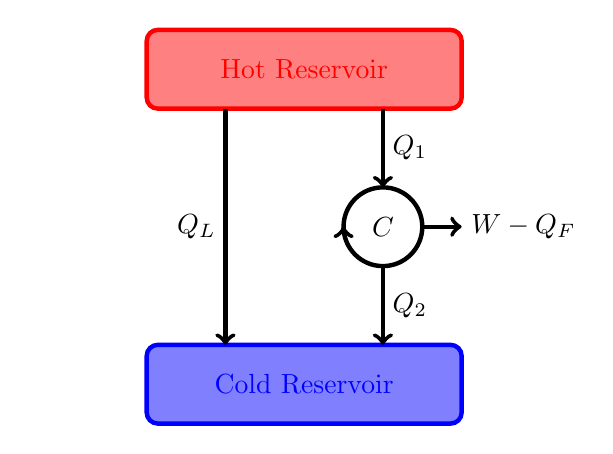
\begin{tikzpicture}
            \tikzstyle{hot} = [color=red, ultra thick, fill=red!50!white, rounded corners]
            \tikzstyle{cold} = [color=blue, ultra thick, fill=blue!50!white, rounded corners]
            \tikzstyle{engine} = [ultra thick, rounded corners]
            \draw[hot] (0, 4) rectangle (4, 5);
            \draw[cold] (0, 0) rectangle (4, 1);
            \draw[engine] (3, 2.5) circle[radius=0.5cm];
            \draw[engine, ->] (2.5, 2.49) -- (2.5, 2.5);
            \node at (3, 2.5) {\(C\)};
            \node[cold] at (2, 0.5) {Cold Reservoir};
            \node[hot] at (2, 4.5) {Hot Reservoir};
            \draw[engine, ->] (3, 4) -- (3, 3);
            \draw[engine, ->] (3, 2) -- (3, 1);
            \draw[engine, ->] (3.5, 2.5) -- (4, 2.5);
            \node[right] at (3, 3.5) {\(Q_1\)};
            \node[right] at (3, 1.5) {\(Q_2\)};
            \node[right] at (4, 2.5) {\(W - Q_F\)};
            \draw[engine, ->] (1, 4) -- (1, 1);
            \node[left] at (1, 2.5) {\(Q_L\)};
            \node[left] at (0, 2.5) {\hphantom{\(W - Q_f\)}};
        \end{tikzpicture}
        \caption{A real engine as a Carnot engine with inefficiencies.}
        \label{fig:real engine}
    \end{figure}
    The Kelvin-Planck statement of the second law means that \(Q_F > 0\) and the Clausius statement of the second law means that \(Q_L > 0\).
    The efficiency is
    \[\eta = \frac{W - Q_F}{Q_1 + Q_L} < \frac{W}{Q_1}\]
    so we see that a real engine must always be less efficient than an ideal engine.
    
    \section{Entropy}
    \subsection{The Clausius Inequality}
    \begin{figure}[ht]
        \centering
        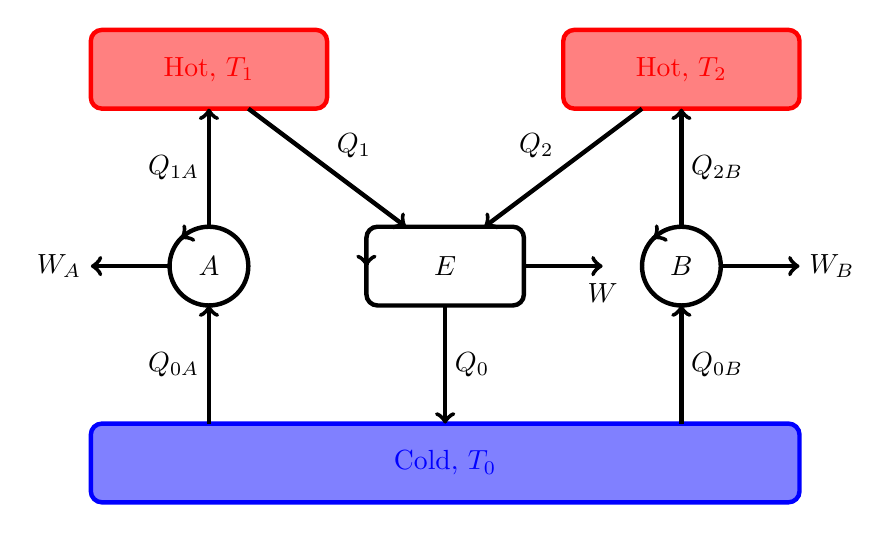
\begin{tikzpicture}
            \tikzstyle{hot} = [color=red, ultra thick, fill=red!50!white, rounded corners]
            \tikzstyle{cold} = [color=blue, ultra thick, fill=blue!50!white, rounded corners]
            \tikzstyle{engine} = [ultra thick, rounded corners]
            \draw[engine] (0.5, 0.5) circle[radius=0.5cm];
            \draw[engine] (2.5, 0) rectangle (4.5, 1);
            \draw[engine] (6.5, 0.5) circle[radius=0.5cm];
            \node at (0.5, 0.5) {\(A\)};
            \node at (3.5, 0.5) {\(E\)};
            \node at (6.5, 0.5) {\(B\)};
            \draw[engine, ->] (0.146, 0.853) -- (0.143, 0.851);
            \draw[engine, ->] (2.5, 0.51) -- (2.5, 0.5);
            \draw[engine, ->] (6.146, 0.853) -- (6.143, 0.851);
            \draw[engine, ->] (0, 0.5) -- (-1, 0.5);
            \node[left] at (-1, 0.5) {\(W_A\)};
            \draw[engine, ->] (4.5, 0.5) -- (5.5, 0.5);
            \node[below] at (5.5, 0.4) {\(W\)};
            \draw[engine, ->] (7, 0.5) -- (8, 0.5);
            \node[right] at (8, 0.5) {\(W_B\)};
            \draw[cold] (-1, -2.5) rectangle (8, -1.5);
            \node[cold] at (3.5, -2) {Cold, \(T_0\)};
            \draw[hot] (-1, 2.5) rectangle (2, 3.5);
            \node[hot] at (0.5, 3) {Hot, \(T_1\)};
            \draw[hot] (5, 2.5) rectangle (8, 3.5);
            \node[hot] at (6.5, 3) {Hot, \(T_2\)};
            \draw[engine, ->] (0.5, 1) -- (0.5, 2.5);
            \draw[engine, ->] (6.5, 1) -- (6.5, 2.5);
            \node[left] at (0.5, 1.75) {\(Q_{1A}\)};
            \node[right] at (6.5, 1.75) {\(Q_{2B}\)};
            \draw[engine, ->] (3.5, 0) -- (3.5, -1.5);
            \node[right] at (3.5, -0.75) {\(Q_0\)};
            \draw[engine, ->] (0.5, -1.5) -- (0.5, 0);
            \node[left] at (0.5, -0.75) {\(Q_{0A}\)};
            \draw[engine, ->] (6.5, -1.5) -- (6.5, 0);
            \node[right] at (6.5, -0.75) {\(Q_{0B}\)};
            \draw[engine, ->] (1, 2.5) -- (3, 1);
            \draw[engine, ->] (6, 2.5) -- (4, 1);
            \node[above right] at (2, 1.75) {\(Q_1\)};
            \node[above left] at (5, 1.75) {\(Q_2\)};
        \end{tikzpicture}
        \caption{The setup for demonstrating Clausius' inequality}
        \label{fig:clausius inequality}
    \end{figure}
    Consider the setup in figure~\ref{fig:clausius inequality}.
    \(A\) and \(B\) are Carnot refrigerators ans \(E\) is an engine.
    There are two hot heat reservoirs at temperatures \(T_1\) and \(T_2\) and a cold heat reservoir at temperature \(T_0\).
    We adjust the engines so that there is no net heat flow to the hot heat reservoirs, that is
    \[Q_{1A} = Q_1,\qquad\text{and}\qquad Q_{2B} = Q_2.\]
    The net heat flow out of the cold reservoir is
    \[Q_{0A} + Q_{0B} - Q_0.\]
    We expect this to be negative (i.e. heat is entering the cold reservoir).
    
    We consider as a system both fridges and the engine.
    The total work done by the system is
    \[W - (W_A + W_B).\]
    We adjust the engine so that there is not heat flow into or out of the heat reservoirs.
    Hence the internal energy is a constant so \(Q_T = W_T\) where \(Q_T\) is the total heat absorbed by the system and \(W_T\) is the total work done by the system (following the engine sign convention).
    Hence we have
    \[Q_{0A} + Q_{0B} - Q_0 = W - (W_A + W_B).\]
    This will violate the Kelvin-Planck statement of the second law unless
    \[W \le W_A + W_B,\qquad\text{and}\qquad Q_{0A} + Q_{0B} - Q_0 \le 0.\]
    Using the efficiency of the Carnot refrigerators we know that
    \[\frac{Q_{1A}}{Q_{0A}} = \frac{T_1}{T_0} \implies Q_{0A} = Q_1\frac{T_0}{T_1},\]
    and similarly
    \[Q_{0B} = Q_2\frac{T_0}{T_2}.\]
    The heat leaving the cold reservoir is
    \[Q_{0A} + Q_{0B} - Q_0 = \left(\frac{Q_1}{T_1} - \frac{Q_2}{T_2}\right)T_0 - Q_0 \le 0.\]
    Hence
    \[\frac{Q_1}{T_1} + \frac{Q_2}{T_2} - \frac{Q_0}{T_0} \le 0.\]
    We now consider heat inputs, \(q_i\), into the working substance of the engine.
    The engine absorbs \(q_1 = Q_1\) and \(q_2 = Q_2\) from the hot reservoirs and returns heat \(Q_0\) to the cold reservoir so \(q_0 = -Q_0\).
    The inequality above then becomes
    \[\frac{q_1}{T_1} + \frac{q_2}{T_2} + \frac{q_0}{T_0} \le 0.\]
    This generalises to any number of engines and refrigerators.
    \[\sum_i \frac{q_i}{T_i} \le 0.\]
    Be careful, \(T_i\) are the temperatures of the reservoirs with which heat is exchanged, not the temperatures of the system.
    
    In the limit where each engine absorbs only an infinitesimal amount of heat, \(\ddbar{q}\), from a large number of reservoirs all at temperature \(T\) this becomes
    \[\int \frac{\ddbar{q}}{T} \le 0.\]
    This is the \define{Clausius inequality}.
    Be careful, \(T\) is the temperature of the surroundings, not the system.
    
    \subsection{Entropy}
    If we apply the Clausius inequality to a reversible system something interesting happens.
    For a reversible process the system and surroundings must be in equilibrium so the temperature of the system, \(T_\sys\), is the same as the temperature of the surroundings, \(T_\surr\).
    Performing the process forward the Clausius inequality must hold so
    \[\int\frac{\ddbar{q_R}}{T} \le 0.\]
    However since this is a reversible process we can also perform it in to opposite direction.
    If we do this then the heat absorbed in each infinitesimal stage is \(-\ddbar{q_R}\) but \(T\) is the same so the Clausius inequality becomes
    \[-\int\frac{\ddbar{q_R}}{T} \le 0.\]
    The only way that both of these can hold is if
    \[\int\frac{\ddbar{q_R}}{T} = 0.\]
    
    Consider a reversible cycle from state \(i\) to state \(f\) and back to \(i\) along path 1 from \(i\) to \(f\) and path 2 from \(f\) to \(i\).
    We can split the integral at \(i\) and \(f\) and we have
    \[\oint \frac{\ddbar{q_R}}{T} = \int_{i~\text{path 1}}^{f} \frac{\ddbar{q_R}}{T} + \int_{f~\text{path 2}}^{i} \frac{\ddbar{q_R}}{T} = 0\]
    Hence
    \[\int_{i~\text{path 1}}^{f} \frac{\ddbar{q_R}}{T} = -\int_{f~\text{path 2}}^{i} \frac{\ddbar{q_R}}{T} = \int_{i~\text{path 2}}^{f} \frac{\ddbar{q_R}}{T}.\]
    This shows that this integral is independent of the path.
    This means that \(\ddbar{q_R}/T\) is an exact differential even though \(\ddbar{q_R}\) is not.
    There must, therefore, be a state function, \(S\), such that
    \[\Delta S = S_f - S_i = \int_i^f \dd{S} = \int_i^f \frac{\ddbar{q_R}}{T}.\]
    We call this state function entropy.
    Notice that this equation only defines a change in entropy.
    It doesn't give us a point where \(S = 0\) and it doesn't tell us what physical property entropy is a measure of.
    
    If path 1 were instead irreversible then the Clausius inequality is
    \[\oint \frac{\ddbar{q}}{T} = \int_{i~\text{path 1}}^{f} \frac{\ddbar{q}}{T} + \int_{f~\text{path 2}}^{i} \frac{\ddbar{q_R}}{T} \le 0.\]
    This implies that
    \[\int_{i~\text{path 1}}^{f} \frac{\ddbar{q}}{T} \le -\int_{f~\text{path 2}}^{i} \frac{\ddbar{q_R}}{T} = \int_{i~\text{path 2}}^{f} \frac{\ddbar{q_R}}{T} = \Delta S.\]
    Note that even though this is an irreversible process we can still do the integral as \(T\) is the temperature of the surroundings and \(\ddbar{q}\) is the heat exchanged with the surroundings and these are defined quantities even though the temperature of the system may not be defined.
    What this means is that the change in entropy for an irreversible process is always less than the change in entropy for an equivalent reversible process, that is
    \[\int_i^f\frac{\ddbar{q}}{T} \le \int_i^f \dd{S},\]
    with equality if and only if the integral on the left is performed over some reversible process.
    
    \begin{example}\label{exa:heating water}
        Water at \SI{20}{\degreeCelsius} is placed in thermal contact with a heat reservoir at \SI{100}{\degreeCelsius}.
        The water is heated irreversibly at constant pressure to an equilibrium state at \SI{100}{\degreeCelsius}.
        What is the change in entropy of the water and of the surroundings?
        
        We consider the water as the system.
        The process is irreversible so we work with an alternative, reversible, process.
        The surroundings in this reversible process are a series of heat reservoirs each at a slightly higher temperature.
        This heats the water slowly in a way that is reversible.
        At each intermediate step in this process there is a reversible transfer of heat, \(\dd{Q} = C_P\dd{T}\), from the surroundings to the system.
        The change in entropy of this intermediate step is then
        \[\dd{S} = \frac{\dd{Q}}{T} = \frac{C_P\dd{T}}{T}.\]
        The total entropy change is then
        \[\Delta S^\sys = C_p\int_{T_i}^{T_f}\frac{\dd{T}}{T} = C_P\ln\left(\frac{T_f}{T_i}\right) \approx 0.241C_P.\]
        
        For the change in entropy of the surroundings we again consider an alternative, reversible, process.
        This time the process is a series of heat reservoirs, each slightly cooler than the last, which represents the heat transferred to the system.
        The total heat transferred is
        \[-C_P(T_f - T_i)\]
        and the change in entropy is
        \[\Delta S^\surr = \frac{C_P(T_f - T_i)}{T_f} \approx -0.21448C_P.\]
        The total entropy change is then
        \[\Delta S^\tot = \Delta S^\sys + \Delta S^\surr = 0.02693C_P > 0.\]
    \end{example}
    
    Consider an adiabatic, thermally isolated system.
    Then \(T\) is a constant and \(\ddbar{q} = 0\).
    Thus \(\dd{S} \ge 0\) where equality holds only for a reversible process.
    This is a statement that entropy never decreases.
    
    We now have four equivalent statements of the second law of thermodynamics:
    \begin{itemize}
        \item Heat can't flow from a cooler reservoir to a hotter reservoir.
        \item Heat cannot be converted to work with \SI{100}{\percent} efficiency.
        \item Reversible cycles are the most efficient engines possible.
        \item Entropy cannot decrease.
    \end{itemize}
    We can think of heat as the lowest form of energy.
    All forms of energy tend towards heat as time progresses.
    This is a statistical phenomenon.
    There are more ways for energy to be heat, that is the motion of particles, than any other form of energy.
    Therefore heat is the most likely form of energy.
    
    The second law is the only fundamental equation in physics which violates \gls{cpt} symmetry.
    We use this to define a `forward' direction in time.
    
    \section{The Central Equation of Thermodynamics}
    If we combine the first law,
    \[\dd{U} = \ddbar{Q} + \ddbar{W},\]
    and the definition of entropy,
    \[\dd{S} = \frac{\ddbar{Q}}{T},\]
    along with the mechanical work done, \(-P\dd{V}\), compressing a fluid, we get the \define{central equation of thermodynamics}:
    \[\dd{U} = T\dd{S} - P\dd{V}.\]
    This is useful as it involves only state variables.
    This means that we can integrate it along any path.
    For an irreversible process we can find an equivalent reversible process along which to integrate.
    This also gives us \(T\dd{S} = \dd{U} + P\dd{V}\) which is an easier way to measure \(\dd{S}\) than the original definition of \(\ddbar{Q}/T\).
    
    An extensive property of a material is one that depends on how much of the material there is, such as volume or internal energy.
    Contrastingly an intensive property of a material is one that doesn't depend on how much of the material there is, such as density or temperature.
    Since the central equation gives us the entropy in terms of the extensive properties \(U\) and \(V\) the entropy must also be an extensive property.
    
    This equation can be made more general if we consider different kinds of work.
    For example, if a charge, \(Z\), is moved by an emf \(\emf\), then the work done is \(\emf\dd{Z}\).
    The central equation is then
    \[\dd{U} = T\dd{S} - P\dd{V} + \emf\dd{Z}.\]
    If instead we consider a rubber band of length \(L\) being stretched by a force, \(F\), then the work done in stretching the rubber band dominates and the central equation becomes
    \[\dd{U} = T\dd{S} + F\dd{L}.\]
    
    \subsection{Entropy of an Ideal Gas}
    We showed in equation~\ref{eqn:dU = C_VdT ideal gas} that for an ideal gas \(\dd{U} = C_V\dd{T}\).
    Using this, and the ideal gas equation, the central equation becomes
    \[\dd{S} = C_V\frac{\dd{T}}{T} + nRT\frac{\dd{V}}{V} = C_V\frac{\dd{T}}{T} + N\boltzmann\frac{\dd{V}}{V}.\]
    If we look at values per mole this becomes
    \[\dd{s} = c_V\frac{\dd{T}}{T} + R\frac{\dd{v}}{v}\]
    where lowercase symbols have the same meaning as their uppercase counter parts but per mole.
    Integrating this gives
    \[s = c_V\ln T + R\ln v + s_0\]
    where \(s_0\) is some constant of integration.
    
    This breaks down as \(T \to 0\) as \(s\to-\infty\).
    This is more than just the fact that the ideal gas equation makes several assumptions and also that kinetic theory breaks down at low temperatures.
    Fundamentally the reason this doesn't work is that, as we will see later, entropy is about counting things and for that things need to be discretised.
    
    \subsection{Entropy change in Joule Expansion}
    In free expansion of an ideal gas there is no work done or heat exchanged.
    Hence \(\dd{U} = \ddbar{Q} + \ddbar{W} = 0\).
    This means the internal energy is constant.
    Since the internal energy of an ideal gas is a function only of its temperature this means that the temperature must be constant and so \(\dd{T} = 0\).
    The volume however does change.
    Therefore there is a change in entropy:
    \[\dd{s} = c_V\frac{\dd{T}}{T} + R\frac{\dd{v}}{v} = R\frac{\dd{v}}{v}.\]
    Integrating this from initial volume \(v_i\) to final volume \(v_f\) we get
    \[\Delta s = s_f - s_i = \int_{s_i}^{s_f}\dd{s} = R\int_{v_i}^{v_f}\frac{\dd{v}}{v} = R\ln\left(\frac{v_f}{v_i}\right)\]
    \[\implies v_f = v_ie^{(s_f - s_i)/R}.\]
    
    \begin{example}
        Consider the same setup as example~\ref{exa:heating water}.
        Water is heated from \SI{20}{\degreeCelsius} to \SI{100}{\degreeCelsius} at a constant pressure in an irreversible way.
        We have already seen one method for calculating the entropy and here we will discuss two more.
        Recall that the method that we have seen is to directly calculate
        \[\Delta S = \int_i^f \frac{\dd{q_R}}{T} = \int_i^f \frac{C_p\dd{T}}{T}\]
        for some alternative reversible process.
        
        The second method we can use is to integrate the central equation:
        \[\Delta S = \int_i^f \frac{\dd{U}}{T} + \int_i^f \frac{P}{T}\dd{V}.\]
        To do this we expand \(\dd{U}\) and \(\dd{V}\) in terms of \(P\) and \(T\).
        We choose \(P\) and \(T\) as \(P\) is constant and \(T\) is the variable that we are interested in changing.
        We get
        \[\Delta S = \int_i^f \frac{1}{T}\left[\pdvconst{U}{T}{P}\dd{T} + \pdvconst{U}{P}{T}\dd{P}\right] + \int_i^f \frac{P}{T}\left[\pdvconst{V}{T}{P}\dd{T} + \pdvconst{V}{P}{T}\dd{P}\right].\]
        Since pressure is constant this reduces to
        \begin{align*}
            \Delta S &= \int_i^f \frac{1}{T} \pdvconst{U}{T}{P}\dd{T} + \int_i^f \frac{P}{T} \pdvconst{V}{T}{P}\dd{T}\\
                &= \int_i^f \frac{1}{T} \left[\pdvconst{U}{T}{P} + P\pdvconst{V}{T}{P}\right]\\
                &= \int_i^f \frac{1}{T} \left(\pdv{T}[U + PV]\right)_{P}\dd{T}\\
                &= \int_i^f \frac{1}{T} \pdvconst{H}{T}{P}\dd{T}.
        \end{align*}
        Comparing this to the result we got with the first method we see that
        \[\pdvconst{H}{T}{P} = C_P.\]
        
        The third method we can use is to use the enthalpy for a constant pressure process:
        \[H = U + PV\]
        Differentiating we get
        \[\dd{H} = \dd{U} + P\dd{V} + V\dd{P}.\]
        Substituting for \(\dd{U}\) with the central equation we get
        \[\dd{H} = T\dd{S} - P\dd{V} + P\dd{V} + V\dd{P} = T\dd{S} + V\dd{P}.\]
        At constant pressure this becomes
        \[\dd{H_P} = T\dd{S_P}.\]
        Integrating this gives
        \[\int_i^f\dd{S_P} = \int\frac{1}{T}\dd{H_P}.\]
        Writing \(H = H(T, P)\) we see that
        \[\dd{H} = \pdvconst{H}{T}{P}\dd{T} + \pdvconst{H}{P}{T}\dd{P} = C_P\dd{T} + \pdvconst{H}{P}{T}\dd{P}.\]
        At constant pressure this becomes
        \[\dd{H_P} = C_P\dd{T}.\]
        Integrating this gives
        \[\int_i^f\dd{S_P} = \int_i^f\frac{1}{T}\dd{H_P} = \int_i^f\frac{C_P}{T}\dd{T},\]
        as we found previously.
    \end{example}
    These three methods are the most common approaches to calculating the entropy in a thermodynamics problem:
    \begin{enumerate}
        \item Try to define a process, or an alternative reversible process if the process in question is irreversible.
        This is usually the longest way to solve a problem but is mathematically the simplest.
        \item Integrate the central equation with the correct work term and with careful consideration of what is held constant and what isn't.
        This is often relatively quick but mathematically trickier.
        \item Use the `correct' thermodynamic variable.
        For example at constant pressure the enthalpy often gives useful values.
        This is why chemists like enthalpy so much.
        This is fast if we know the `correct' variable to use but not much use if we don't.
    \end{enumerate}
    
    \subsection{Entropy Change in the Universe}
    Heat water from \(T\) to \(T + \Delta T\).
    The entropy change of the water and surroundings are
    \[\Delta S_\sys = C_P \ln\left(\frac{T + \Delta T}{T}\right),\]
    and
    \[\Delta S_\surr = C_P\frac{\Delta T}{T}.\]
    These were calculated in example~\ref{exa:heating water}.
    If we define \(x = \Delta T/T\) then the total entropy change is
    \[\Delta S_\tot = C_P[x - \ln(1 + x)].\]
    This is non-negative for all \(x > -1\).
    We see that for positive \(T\) the entropy must increase.
    
    \begin{example}
        Consider an emf, \(\emf\), driving a current, \(I\), through a resistor, \(R\), in an adiabatic box.
        The power output is \(I^2R\).
        No heat or mechanical work is exchanged with the surroundings so the total internal energy change in time \(\Delta t\) is
        \[\Delta U = I^2R\Delta t.\]
        Electrical work is dissipated irreversibly as heat,
        \[\Delta U = C_V\Delta T,\]
        which must all go to heating up the box since it is adiabatic.
        The change in temperature can be calculated:
        \[\Delta T = \frac{I^2R\Delta t}{C_V}.\]
        What is the change in entropy?
        
        Volume is constant so \(\dd{V} = 0\), therefore the central equation becomes
        \[\dd{S} = \frac{\dd{U}}{T} \implies \dd{S} = \frac{C_V\dd{T}}{T}.\]
        Integrating gives us
        \[\Delta S = \int_{T}^{T + \Delta T} \frac{C_V}{T}\dd{T}.\]
        Alternatively we could have defined an equivalent reversible heating process and found that
        \[\Delta S = \int_{T}^{T + \Delta T}\frac{\ddbar{q_R}}{T} = \int_{T}^{T + \Delta T}\frac{C_V\dd{T}}{T}.\]
        Either way the entropy change is
        \[\Delta S = C_V\ln\left(1 + \frac{I^2R\Delta t}{TC_V}\right).\]
        Again as \(T \to 0\) we now have \(\Delta S \to\infty\).
        So this breaks down when temperatures are near zero.
    \end{example}
    
    \subsection{Statistical Entropy}
    \textit{This section will be expanded upon in the statistical mechanics part of this course.}
    
    The total entropy can be defined as
    \[S = \boltzmann\ln\Omega\]
    where \(\Omega\) is the total number of ways it is possible to arrange the system.
    For example, consider Joule expansion where one box, \(A\), full of gas is allowed to expand freely into a second box, \(B\), which is initially under a vacuum.
    After this expansion the probability that any one atom is in box \(A\) is \(1/2\).
    The probability that all atoms are in box \(A\) is \(1/2^N\) where \(N\sim N_A\) is the number of atoms, clearly this is incredibly unlikely.
    The probability that \SI{50}{\percent} of the atoms are in box \(A\) is
    \[{N\choose N/2} \frac{1}{2^N}.\]
    In general the probability that \(r\) of the atoms are in box \(A\) is
    \[{N\choose r}\frac{1}{2^N}.\]
    The maximum value of this comes at \(r = N/2\) which means that the state where the atoms are evenly distributed between the two boxes is the most likely.
    This is also the highest entropy state since it is more likely precisely because there are more arrangements of the system that lead to this arrangement.
    
    The number of possible states with all particles
    \begin{enumerate}
        \item in A is \(\Omega(N, V, E)\)
        \item in \(A\) or \(B\) is \(\Omega(N, 2V, E)\).
    \end{enumerate}
    If all accessible microstates are equally likely then
    \[\frac{\Omega_A}{\Omega_{A+B}} = \frac{\Omega(N, V, E)}{\Omega(N, 2V, E)} = \frac{1}{2^N}.\]
    
    We can justify the form of this definition of entropy heuristically.
    Suppose that there exists a function, \(f\), such that \(f(\Omega) = S\).
    Entropy, being an extensive property, is additive.
    That is if a system is formed from two subsystems with entropies \(S_1\) and \(S_2\) then the total entropy is
    \[S = S_1 + S_2.\]
    Permutations on the other hand are multiplicative.
    That is if a system is formed from two subsystems which can be arranged in \(\Omega_1\) and \(\Omega_2\) ways then the total number of arrangements of the whole system is
    \[\Omega = \Omega_1\Omega_2.\]
    Hence we must have
    \[f(\Omega) = f(\Omega_1\Omega_2) = f(\Omega_1) + f(\Omega_2) = S_1 + S_2.\]
    This holds if \(f(\omega) = \ln\Omega\).
    Thus for fixed energy, \(E\), we define
    \[S = \boltzmann\ln\Omega.\]
    One important factor that comes from this is that \(\Omega\) involves counting things which means that said `things' need to be discretised which leads to quantum mechanics.
    
    \section{Thermodynamic Potentials}
    A mechanical equilibrium is reached when the energy is minimised.
    A thermodynamic equilibrium is reached when entropy is maximised.
    We define the free energy as the thermodynamic variable that is minimised to reach a thermodynamic equilibrium.
    This is useful as the entropy is often difficult to measure and therefore not very useful for practical applications.
    We have already met two such variables that we can minimise for equilibrium and we will introduce some more.
    These variables are called \define{free energies} or \define{thermodynamic potentials}.
    Which thermodynamic potential we work with depends on which state variables we are working with.
    The thermodynamic potentials are themselves state variables and therefore can be written as a function of two other state variables.
    Typically we choose the two variables that simplify the maths, which often means one variable that is held constant and one variable that we control the change in.
    The thermodynamic potentials and the natural variables to work in are given in table~\ref{tab:the thermodynamic potentials}.
    \begin{table}[ht]
        \centering
        \begin{tabular}{lll}\hline
            Potential & Differential & Natural Units\\\hline
            Internal energy, \(U\) & \(\dd{U} = T\dd{S} - P\dd{V}\) & \(S\), \(V\)\\
            Enthalpy, \(H = U + PV\) & \(\dd{H} = T\dd{S} + V\dd{P}\) & \(S\), \(P\)\\
            Helmholtz free energy\tablefootnote{sometimes denoted \(A\)}, \(F = U - TS\) & \(\dd{F} = -P\dd{V} - S\dd{T}\) & \(T\), \(V\)\\
            Gibbs free energy, \(G = H - TS\) & \(\dd{G} = V\dd{P} - S\dd{T}\) & \(T\), \(P\)\\\hline
        \end{tabular}
        \caption{The thermodynamic potentials}
        \label{tab:the thermodynamic potentials}
    \end{table}
    Which potential we choose depends on what the situation is.
    In chemistry most experiments are open to the atmosphere so \(P\) is constant.
    The temperature is also readily measured and controlled.
    This means that often the Gibbs free energy, \(G\), is the best potential to use.
    In physics we often work with \(S\) and \(T\) as constants, for example, a pendulum swinging.
    Therefore we work with internal energy, \(\dd{U} = -\ddbar{W}\), for some appropriate expression of work.
    
    In mechanics we often start with a Hamiltonian, \(\hamiltonian\), and we assume that \(\hamiltonian\) is the sum of the kinetic and potential energies.
    This assumes that we have boundary conditions of \(S\) and \(V\) being constant and therefore we can use \(\hamiltonian = U\).
    If instead we study air as a sound wave passes then \(S\) and \(P\) are the variables of interest so we should use \(\hamiltonian = H\).
    If we study reagents dissolved in water then we have \(T\) and \(V\) being the variables of interest so we should use \(\hamiltonian = F\).
    If we study water exposed to the atmosphere then we have \(T\) and \(P\) being the variables of interest so we should use \(\hamiltonian = G\).
    In general we look at any boundaries in the system and at what variables are either constant or can change over those boundaries.
    
    \subsection{Maxwell Relations}
    State functions can usually be written as function of two independent variables.
    Therefore there must be a relationship between the state functions.
    The equation of state is one such relationship that is material specific.
    There are also relationships that are general and true due to the mathematical nature of the state variables.
    In particular we can use the fact that the potentials are state variables and therefore represented by nice functions of their natural variables and partial derivatives commute.
    This allows us to derive four relations called the Maxwell relations.
    
    We start with
    \[\dd{U} = T\dd{S} - P\dd{V}.\]
    Taking a derivative with respect to \(V\) at constant entropy we have
    \[\pdvconst{U}{V}{S} = -P.\]
    Taking a derivative with respect to \(S\) at constant volume we have
    \[\pdvsec{U}{S_V}{V_S} = -\pdvconst{P}{S}{V}.\]
    Since partial derivatives commute if we compute this in the other direction we must get the same result:
    First
    \[\pdvconst{U}{S}{V} = T,\]
    then
    \[\pdvsec{U}{V_S}{S_V} = \pdvconst{T}{V}{S}.\]
    So we conclude
    \[\pdvconst{T}{V}{S} = -\pdvconst{P}{S}{V}.\]
    
    Next we start with
    \[\dd{H} = T\dd{S} + V\dd{P}.\]
    \begin{align*}
        &\implies \pdvconst{H}{S}{P} = T \implies \pdvsec{H}{P_S}{S_P} = \pdvconst{T}{P}{S}\\
        &\implies \pdvconst{H}{P}{S} = V \implies \pdvsec{H}{S_P}{P_S} = \pdvconst{V}{S}{P}\\
        &\implies \pdvconst{T}{P}{S} = \pdvconst{V}{S}{P}.
    \end{align*}

    Next we start with
    \[\dd{F} = -P\dd{V} - S\dd{T}\]
    \begin{align*}
        &\implies \pdvconst{F}{V}{T} = -P \implies \pdvsec{F}{T_V}{V_T} = -\pdvconst{P}{T}{V}\\
        &\implies \pdvconst{F}{T}{V} = -S \implies \pdvsec{F}{V_T}{T_V} = -\pdvconst{S}{V}{T}\\
        &\implies \pdvconst{P}{T}{V} = \pdvconst{S}{V}{T}.
    \end{align*}

    Finally we start with
    \[\dd{G} = V\dd{P} - S\dd{T}\]
    \begin{align*}
        &\implies \pdvconst{G}{P}{T} = V \implies \pdvsec{G}{T_P}{P_T} = \pdvconst{V}{T}{P}\\
        &\implies \pdvconst{G}{T}{P} = -S \implies \pdvsec{G}{P_T}{T_P} = -\pdvconst{S}{P}{T}\\
        &\implies \pdvconst{V}{T}{P} = -\pdvconst{S}{P}{T}.
    \end{align*}
    
    All four relations are:
    \begin{align*}
        \hphantom{-}\pdvconst{T}{V}{S} &= -\pdvconst{P}{S}{V} = \pdvsec{U}{S}{V} \\
        \hphantom{-}\pdvconst{T}{P}{S} &= \hphantom{-}\pdvconst{V}{S}{P} = \pdvsec{H}{S}{P} \\
        \hphantom{-}\pdvconst{S}{V}{T} &= \hphantom{-}\pdvconst{P}{T}{V} = \pdvsec{F}{T}{V} \\
        -\pdvconst{S}{P}{T} &= \hphantom{-}\pdvconst{V}{T}{P} = \pdvsec{G}{T}{P} \\
    \end{align*}
    
    \subsection{Remembering the Thermodynamic Potentials and Maxwell Relations}
    In the Maxwell relations the natural variables of the relevant potential are the ones that appear in the denominator.
    For a derivative like
    \[\pdvconst{x}{y}{z}\]
    \(xz\) has units of energy.
    
    The following mnemonic gives us the potentials and Maxwell's relations:
    \begin{displayquote}
        \textbf{G}ood \textbf{P}hysicists \textbf{H}ave \textbf{S}tudied \textbf{U}nder \textbf{V}ery \textbf{F}ine \textbf{T}eachers.
    \end{displayquote}
    We use this to remember the potentials and state variables in the order \(G, P, H, S, U, V, F, T\).
    We then place these anticlockwise around a square as shown in figure~\ref{fig:mnemonic}.
    \begin{figure}[ht]
        \centering
        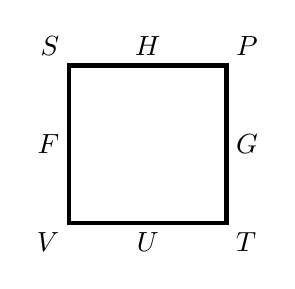
\begin{tikzpicture}
            \draw[ultra thick] (0, 0) rectangle (2, 2);
            \node[right] at (2, 1) {\(G\)};
            \node[above right] at (2, 2) {\(P\)};
            \node[above] at (1, 2) {\(H\)};
            \node[above left] at (0, 2) {\(S\)};
            \node[left] at (0, 1) {\(F\)};
            \node[below left] at (0, 0) {\(V\)};
            \node[below] at (1, 0) {\(U\)};
            \node[below right] at (2, 0) {\(T\)};
        \end{tikzpicture}
        \caption{Mnemonic for remembering thermodynamic potentials and Maxwell relations.}
        \label{fig:mnemonic}
    \end{figure}
    The natural variables for describing a potential are then the two variables on the same line as it, for example \(H = H(S, P)\).
    This means that we can write
    \[\dd{H} = \text{sign}\,\text{const}\dd{S} + \text{sign}\,\text{const}\dd{P}.\]
    The constants are given by the diagonal opposite of the state variables that make up the differential:
    \[\dd{H} = \text{sign}\,T\dd{S} + \text{sign}\,V\dd{P}.\]
    Finally we get the sign by drawing an arrow from the constant to the differential.
    If the arrow is up then the sign is positive, if it is down then the sign is negative, the arrows are shown in figure~\ref{fig:mnemonic for H}:
    \[\dd{H} = T\dd{S} + V\dd{P}.\]
    \begin{figure}[ht]
        \centering
        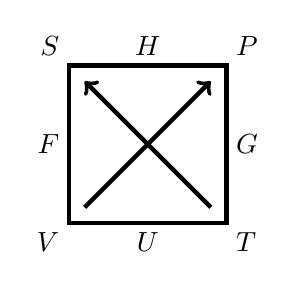
\begin{tikzpicture}
            \draw[ultra thick] (0, 0) rectangle (2, 2);
            \node[right] at (2, 1) {\(G\)};
            \node[above right] at (2, 2) {\(P\)};
            \node[above] at (1, 2) {\(H\)};
            \node[above left] at (0, 2) {\(S\)};
            \node[left] at (0, 1) {\(F\)};
            \node[below left] at (0, 0) {\(V\)};
            \node[below] at (1, 0) {\(U\)};
            \node[below right] at (2, 0) {\(T\)};
            \draw[ultra thick, ->] (0.2, 0.2) -- (1.8, 1.8);
            \draw[ultra thick, ->] (1.8, 0.2) -- (0.2, 1.8);
        \end{tikzpicture}
        \caption{Using the mnemonic to find the thermodynamic potentials.}
        \label{fig:mnemonic for H}
    \end{figure}
    We can get the Maxwell relations for two state variables by picking the two variables that aren't diagonally opposite, for example \(S\) and \(V\).
    We then start with the form
    \[\pdvconst{V}{?}{\text{const}} = \text{sign}\pdvconst{S}{?}{\text{const}}.\]
    We draw arrows along the diagonals from the variables of interest, this is shown in figure~\ref{fig:mnemonic maxwell relations}.
    \begin{figure}[ht]
        \centering
        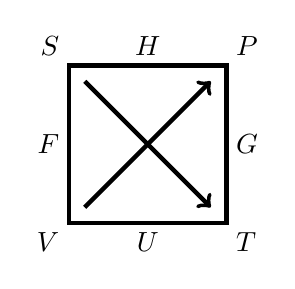
\begin{tikzpicture}
            \draw[ultra thick] (0, 0) rectangle (2, 2);
            \node[right] at (2, 1) {\(G\)};
            \node[above right] at (2, 2) {\(P\)};
            \node[above] at (1, 2) {\(H\)};
            \node[above left] at (0, 2) {\(S\)};
            \node[left] at (0, 1) {\(F\)};
            \node[below left] at (0, 0) {\(V\)};
            \node[below] at (1, 0) {\(U\)};
            \node[below right] at (2, 0) {\(T\)};
            \draw[ultra thick, ->] (0.2, 0.2) -- (1.8, 1.8);
            \draw[ultra thick, ->] (0.2, 1.8) -- (1.8, 0.2);
        \end{tikzpicture}
        \caption{Using the mnemonic to find Maxwell's relations}
        \label{fig:mnemonic maxwell relations}
    \end{figure}
    The thing that is held constant is given by the end of the arrow:
    \[\pdvconst{V}{?}{P} = \text{sign}\pdvconst{S}{?}{T}.\]
    The variable we differentiate with respect to is given by the end of the other arrow:
    \[\pdvconst{V}{T}{P} = \text{sign}\pdvconst{S}{P}{T}.\]
    If both arrows are up or both are down then the sign is positive, else the sign is negative:
    \[\pdvconst{V}{T}{P} = -\pdvconst{S}{P}{T}.\]
    
    \subsection{\texorpdfstring{\(T\dd{S}\)}{TdS} Equations}
    Using these relations we can find the entropy in terms of other, more easily measured variables:
    \[T\dd{S} = c_V\dd{T} + T\pdvconst{P}{T}{V}\dd{v},\]
    \[T\dd{S} = c_P\dd{T} - T\pdvconst{V}{T}{P}\dd{P},\]
    and
    \[T\dd{S} = c_p\pdvconst{T}{V}{P}\dd{v} + c_V\pdvconst{T}{P}{V}\dd{P}.\]
    These are called the \(T\dd{S}\) equations.
    
    \subsection{Gay--Lussac Law}
    The Gay--Lussac law, also known as Amonton's law, is that the ratio of pressure and temperature is a constant, known as the Gay--Lussac constant, \(\gaylussac\):
    \[\gaylussac = \frac{P}{T}.\]
    If we assume an isothermal process then
    \[\gaylussac = \pdvconst{P}{T}{V} = \pdvconst{S}{V}{T}.\]
    This constant, \(\gaylussac\), is a property of the material.
    
    \subsection{Iso-}
    Iso-, from the Greek, \textgreek{ἶσος} (isos) meaning equal, is a prefix usually used to denote that a quantity is constant for a certain process:
    \begin{itemize}
        \item Isotropic -- Equal in all directions,
        \item Isotopic -- Equal element,
        \item Isothermal -- Equal temperature,
        \item Isobaric -- Equal pressure,
        \item Isochoric/Isovolumetric -- Equal volume,
        \item Isenthalpic -- Equal enthalpy,
        \item Isoenergetic -- Equal energy,
        \item Isentropic -- Equal entropy,
        \item Adiabatic -- Equal heat.
    \end{itemize}

    \subsection{Minimising Thermodynamic Potentials}
    We started the section by claiming that minimising the relevant thermodynamic potential was the same as maximising the entropy.
    In this section we will show this for a specific system.
    Suppose a gas, initially at temperature \(T\) and pressure \(P\) is placed in thermal contact with a temperature and pressure reservoir at temperature \(T_0\) and pressure \(P_0\).
    Also the gas and reservoir are adiabatically separated from the rest of the universe and there is a free (meaning able to move) wall between the system and the reservoir.
    Initially the system is out of equilibrium.
    Heat, \(Q\), flows between the system and the reservoir.
    The change in entropy of the surroundings is
    \[\Delta S_0 = -\frac{Q}{T_0}.\]
    The change in volume of the surroundings is
    \[\Delta V_0 = \Delta V = \frac{W}{P_0}.\]
    The second law means
    \[\Delta S_\sys + \Delta S_0 \ge 0.\]
    The first law is
    \[Q = \Delta U + P_0\Delta V.\]
    Combining these we have
    \[\Delta U + P_0\Delta V - T_0\Delta S_0 \le 0.\]
    Since \(P_0\) and \(T_0\) are constant for a pressure and temperature reservoir this can be written as
    \[\Delta(U + PV - TS) \le 0. \implies \Delta(H - TS) \le 0 \implies \Delta G \le 0.\]
    We made no assumptions about which way the system had to move to reach equilibrium so we see that any step that the system makes towards equilibrium will decreases \(G\) therefore the system is in equilibrium when \(G\) is minimised, which is also when the entropy is maximised.
    
    \section{Availability}
    \subsection{General Relation between \texorpdfstring{\(C_P\)}{CP} and \texorpdfstring{\(C_V\)}{CV}}
    For an ideal gas we showed that
    \[C_P - C_V = nR.\]
    We are now ready to find a general relation between \(C_P\) and \(C_V\).
    At a constant volume from the first law we have \(\dd{U} = \ddbar{Q}\) the central equation we have \(\dd{U} = T\dd{S}\).
    Thus
    \[C_V = \pdvconst{Q}{T}{V} = \pdvconst{U}{T}{V} = T\pdvconst{S}{T}{V}.\]
    At constant pressure we have \(\dd{H} = \dd{U} = T\dd{S}\) and so
    \[C_P = \pdvconst{H}{T}{P} = T\pdvconst{S}{T}{P}.\]
    This suggests that we should work with the entropy, \(S = S(T, V)\).
    In this case \(\dd{S}\) is given by
    \[\dd{S} = \pdvconst{S}{T}{V}\dd{T} + \pdvconst{S}{V}{T}\dd{V}.\]
    Differentiating with respect to temperature at constant pressure this becomes
    \[\pdvconst{S}{T}{P} = \pdvconst{S}{T}{V}\pdvconst{T}{T}{P} + \pdvconst{S}{V}{T}\pdvconst{V}{T}{P} = \pdvconst{S}{T}{V} + \pdvconst{S}{V}{T}\pdvconst{V}{T}{P}.\]
    Multiplying by \(T\) we have
    \[C_P = T\pdvconst{S}{T}{P} = T\pdvconst{S}{V}{T} + T\pdvconst{S}{V}{T}\pdvconst{V}{T}{P} = C_V + T\pdvconst{S}{V}{T}\pdvconst{V}{T}{P}.\]
    We now introduce the isobaric thermal expansivity, \(\beta\), defined as
    \[\beta = \frac{1}{V}\pdvconst{V}{T}{P}.\]
    Thus
    \begin{equation}\label{eqn:C_P = C_V + TVbeta dS/dV_T}
        C_P = C_V + TV\beta\pdvconst{S}{V}{T}.
    \end{equation}
    By Maxwell's relations we have
    \[\pdvconst{S}{V}{T} = \pdvconst{P}{T}{V}.\]
    The triple product rule for partial derivatives is that
    \[\pdvconst{x}{y}{z}\pdvconst{y}{z}{x}\pdvconst{z}{x}{y} = -1.\]
    Using this and the reciprocal rule
    \[\frac{1}{\pdvconst{x}{y}{z}} = \pdvconst{y}{x}{z}\]
    we have
    \[\pdvconst{S}{V}{T} = \pdvconst{P}{T}{V} = -\pdvconst{P}{V}{T}\pdvconst{V}{T}{P}.\]
    Introducing the isothermal bulk modulus, \(K\), defined as
    \[K = -V\pdvconst{P}{V}{T}\]
    we have
    \[\pdvconst{S}{V}{T} = -V\pdvconst{P}{V}{T}\frac{1}{V}\pdvconst{V}{T}{P} = K\beta.\]
    Substituting this into equation~\ref{eqn:C_P = C_V + TVbeta dS/dV_T} we have
    \[C_P - C_V = TV\beta\pdvconst{S}{V}{T} = TV\beta^2 K = \frac{TV\beta^2}{\kappa}.\]
    Here we have introduced the isothermal compressibility, \(\kappa = 1/K\), which is more commonly used with gasses whereas \(K\) is more commonly used with solids.
    We see that
    \[C_P - C_V \propto V\]
    which makes sense as it is an extensive property meaning it depends on how much stuff there is.
    For all known substances \(K > 0\) and also \(T > 0\) in kelvins and \(\beta^2 > 0\) for all \(\beta\) so \(C_P - C_V \ge 0\) and \(C_P \ge C_V\).
    This even works if the thermal expansion, \(\beta\), is negative.
    This means that the difference is not due to the work done expanding at constant \(P\) as \(C_P \ge C_V\) even if the material shrinks upon heating, this goes against one of the most common (incorrect) explanations for why \(C_P\) is greater.
    \(C_P = C_V\) at the density maximum of water (which occurs at about \SI{4}{\degreeCelsius} and \SI{1}{\atm}).
    For solids and liquids \(\beta\) is usually small and therefore \(C_P \approx C_V\).
    For this reason we often don't differentiate between \(C_P\) and \(C_V\) and just quote a single value of heat capacity, which is usually \(C_P\).
    
    \subsection{Changes in Heat Capacities}\label{sec:changes in heat capacities}
    The values of \(C_V\) and \(C_P\), even for an ideal gas, depend on the structure of the molecules as the degrees of freedom are important.
    At room temperature however most vibrational degrees of freedom aren't accessible so only translational and rotational degrees of freedom play a part.
    
    One thing that we might want to know is how does \(C_V\) change with volume.
    That is what is
    \[\pdvconst{C_V}{V}{T}?\]
    We can calculate this fairly easily:
    \begin{align*}
        \pdvconst{C_V}{V}{T} &= T\left(\pdv{V}\pdvconst{S}{T}{V}\right)_T\\
        &= T\left(\pdv{T}\pdvconst{S}{V}{T}\right)_V\\
        &= T\left(\pdv{T}\pdvconst{P}{T}{V}\right)_V\\
        &= T\pdvconst[2]{P}{T}.
    \end{align*}
    Here we have used one of Maxwell's relations:
    \[\pdvconst{S}{V}{T} = \pdvconst{P}{T}{V}.\]
    Similarly we can show that
    \[\pdvconst{C_P}{P}{T} = -T\pdvconst[2]{V}{T}{P}.\]
    We can obtain these derivatives directly from the equations of state without even needing to know \(C_V\) and \(C_P\), for example an ideal gas has
    \[V = \frac{nRT}{P} \implies \pdvconst{C_P}{P}{T} = -T\left(\pdv{T}\left(\pdv{T}\frac{nRT}{P}\right)_P\right)_P = \left(\pdv{T}\frac{nR}{P}\right)_P = 0.\]
    Sometimes we can measure
    \[\pdvconst{C_P}{P}{T}\]
    at multiple pressures and integrate to get \(C_P\), or we could find \(C_V\) in a similar way.
    
    One interesting point is that \(C_P\) is infinite at phase transitions as at a phase transition \(\Delta T = 0\) between phases and \(\Delta V \ne 0\).
    Hence
    \[C_P = \pdvconst{Q}{T}{P} = -P\pdvconst{V}{T}{P}\]
    assuming an ideal gas so \(U\) is constant at a phase boundary since \(T\) is constant and \(U = U(T)\).
    The latent heat is
    \[L = \int_{T - \delta T}^{T + \delta T}C_P\dd{T}\]
    where \(T\) is the temperature at which the phase transition occurs and \(\delta T \to 0\).
    We know that \(L\) is finite and therefore we model \(C_P\) with a delta distribution at phase transitions.
    
    \subsection{Why Don't Experiments Work}
    Many classical physics experiments are based on the assumption that
    \[F = -\pdv{U}{x}.\]
    While this is true under ideal conditions things like friction get in the way.
    We can quantify how much using thermodynamics.
    Differentiating the central equation with respect to volume and at constant temperature we have
    \[\pdvconst{U}{V}{T} = T\pdvconst{S}{T}{T} - P = T\pdvconst{P}{T}{V} - P = \frac{T\beta}{\kappa} - P.\]
    Here we have used a Maxwell relation and the definitions of \(\beta\) and \(\kappa\).
    Since pressure is force per unit area we can divide by area to get
    \[\pdvconst{U}{x}{T} = \frac{T\beta}{\kappa A} -F \implies F = -\pdvconst{U}{x}{T} + \frac{T\beta}{\kappa A}.\]
    This extra term compared to the definition of potential energy explains why many experiments don't give quite the expected value.
    
    \subsection{Energy Change with Pressure}
    The energy increases under a pressure change.
    We can show this by differentiation the central equation with respect to pressure and holding \(T\) constant:
    \[\pdvconst{U}{P}{T} = T\pdvconst{S}{P}{T} - P\pdvconst{V}{P}{T} = T\pdvconst{V}{T}{P} - P\pdvconst{V}{P}{T}\]
    where we have used one of Maxwell's relations to get rid of \(S\).
    Identifying various terms this is
    \[\pdvconst{U}{P}{T} = -TV\beta + PV\kappa_T\]
    where \(\kappa_T\) is the isothermal compressibility, defined as
    \[\kappa_T = -\frac{1}{V}\pdvconst{V}{P}{T}.\]
    We can show that
    \[\frac{C_P}{C_V} = \frac{\kappa_T}{\kappa_S}\]
    where \(\kappa_S\) is the adiabatic compressibility, defined as
    \[\kappa_S = -\frac{1}{V}\pdvconst{V}{P}{S}.\]
    This gives us another link between thermal \((C_P/C_V)\) and mechanical \((\kappa_T/\kappa_S)\) properties.
    
    \subsection{Entropy of an Ideal Gas (Again)}
    The entropy per mole of an ideal gas is \(s = s(T, V)\).
    \[\dd{s} = \pdvconst{s}{T}{V}\dd{T} + \pdvconst{s}{V}{T}\dd{V} = c_V\frac{\dd{T}}{T} + \beta K\dd{V}.\]
    This applies to any fluid so far.
    For an ideal gas we have that \(\beta K = R/V\) and \(c_V\) is constant so integrating this we have
    \[s = c_V\ln T + R\ln v + s_0.\]
    Similarly we can show that
    \[s = c_p\ln T - R\ln P + s_0.\]
    So we have related changes in entropy to measurable properties via the equations of state.
    
    \subsection{Availability}
    Given a specific system how much work can we get out?
    The answer depends on the surroundings.
    Suppose that the system is surrounded by a \(T_0, P_0\) reservoir.
    The second law means that
    \[\Delta S_\sys  + \Delta S_\surr \ge 0.\]
    Which is
    \[\Delta S_\sys - \frac{\Delta Q}{T_0 \ge 0}\]
    where \(\Delta Q\) is the heat transferred from the the surroundings to the system.
    The first law for the system means that \(\Delta Q = \Delta U + P_0\Delta V\) and hence
    \[\Delta U + P_0\Delta V - T_0\Delta S \le 0.\]
    We define the availability, \(A\), to be
    \[A = U - T_0S + P_0V.\]
    Note that this is different from the Gibbs free energy as \(T_0\) and \(P_0\) are the temperature and pressure of the surroundings, not the system.
    
    \(A\) depends on the system and surroundings, \(A = A(S, V, P_0, T_0)\).
    We have already seen that spontaneous changes in \(A\) are negative since
    \[\Delta A = \Delta U + P_0\Delta V - T_0\Delta S \le 0.\]
    At equilibrium nothing can change and since \(\Delta A\) can only decrease it must be minimised at equilibrium.
    In differential form
    \[\dd{A} = \dd{U} - T_0\dd{S} + P_0\dd{V}.\]
    At equilibrium we will have \(T_0 = T\) and \(P_0 = P\) and \(\dd{A} = 0\).
    The following scenarios show how useful \(A\) is, at equilibrium by minimising \(A\) with certain conditions we have:
    \begin{align*}
        &T = T_0 & P = P_0 && A &= U - TS + PV && G~\text{minimised}\\
        &T = T_0 & V~\text{const} && A &= U - TS + \text{const} && F~\text{minimised}\\
        &S~\text{const} & V~\text{const} && A &= U + \text{const} && U~\text{minimised}\\
        &S~\text{const} & P = P_0 && A &= U - \text{const} + PV && H~\text{minimised}\\
        &U~\text{const} & V~\text{const} && A &= \text{const} - T_0S && S~\text{maximised}
    \end{align*}
    \(A\) gives us a measure of how far we are from equilibrium.
    
    The work, \(P_0\Delta V\) is used to push back the environment.
    It is wasted.
    The heat transferred could be used to run an engine producing useful work.
    We have
    \[\Delta U = Q - W = Q - W_\text{useful} - P_0\Delta V.\]
    \(Q\)  is the heat transported from the surroundings to the system.
    Rearranging this and substituting in \(Q = T_0\Delta S\) we have
    \[0 = \Delta U + P_0\Delta V - T_0\Delta S + W_\text{useful} = W_\text{useful} - \Delta A.\]
    Therefore the maximum amount of useful work that we can extract is 
    \[W_{\max} = -\Delta A.\]
    This occurs if and only if all changes are reversible.
    In all other cases the work that we can extract is less.
    In differential form we have
    \begin{align*}
        \dd{W_\text{useful}} &\le -\dd{A}\\
        &= -\dd{U} + T_0\dd{S} - P_0\dd{V}\\
        &= -T\dd{S} + P\dd{V} + T_0\dd{S} - P_0\dd{V}\\
        &= (T_0 - T)\dd{S} - (P_0 - P)\dd{V}
    \end{align*}
    so we see that the work we can do is directly related to the difference in pressure and temperature of the system and surroundings.
    
    \section{Free Expansion of a Real Gas}
    In section~\ref{sec:irreversible free expansion and the Joule coefficient} we considered a gas expanding into a vacuum to twice its original volume in a rigid adiabatic container.
    We argued that these properties meant no work was done and no heat was transferred, therefore bu the first law \(\dd{U} = 0\).
    Then we looked at an ideal gas and said that \(\dd{U} = 0\) implies \(\dd{T} = 0\) since for an ideal gas \(U = U(T)\) so if \(U\) is constant \(T\) must be also.
    Finally we defined the Joule coefficient
    \[\mu_J = \pdvconst{T}{V}{U}\]
    such that \(\dd{T} = \mu_J\dd{V}\), which we found by expanding a differential of \(T = T(V, U)\) and setting \(\dd{U} = 0\).
    For an ideal gas \(\mu_J = 0\) since \(\dd{T} = 0\).
    
    We now have enough thermodynamics to reconsider this problem for real gases.
    Since the container is adiabatic the entropy of the surroundings, \(S_0\), is constant, so \(\dd{S_0} = 0\).
    Since the container is rigid the volume of the surroundings, \(V_0\), is constant so \(\dd{V_0} = 0\).
    For the surroundings \(\dd{U} = \ddbar{Q} + \ddbar{W} = 0\) since no work is done and no heat is transferred.
    Turning now to the system we want to know how the change in volume effects the temperature.
    We want to know what
    \[\mu_J = \pdvconst{T}{V}{U}\]
    is since then we know that
    \[\dd{T} = \pdvconst{T}{V}{U}\dd{V} = \mu_J\dd{V}.\]
    Integrating this we have
    \[\Delta T = \int_{V_i}^{V_f}\pdvconst{T}{V}{U}\dd{V} = \int_{V_i}^{V_f}\mu_J\dd{V}.\]
    We can't directly measure \(U\) so we would like to get rid of it.
    To do this we use the partial derivative triple product:
    \[\pdvconst{T}{V}{U} = -\pdvconst{T}{U}{V}\pdvconst{U}{V}{T}.\]
    Identifying
    \[\pdvconst{U}{T}{V} = C_V\]
    and using the reciprocal rule for partial derivatives we have
    \[\pdvconst{T}{V}{U} = -\frac{1}{C_V}\pdvconst{U}{V}{T}.\]
    Differentiating the central equation with respect to \(V\) at constant \(T\) we get
    \[\pdvconst{U}{V}{T} = T\pdvconst{S}{V}{T} - P.\]
    Therefore
    \[\mu_J = \pdvconst{T}{V}{U} = \frac{1}{C_V}\left[P - T\pdvconst{P}{T}{V}\right],\]
    where we have used a Maxwell relation to get rid of the entropy.
    This allows us to calculate \(\mu_J\) from the equation of state, \(U = U(P, T)\).
    For an ideal gas
    \[P = \frac{nRT}{V} \implies \pdvconst{P}{T}{V} = \frac{nR}{V} \implies T\pdvconst{P}{T}{V} = T\frac{nR}{V} = P\]
    so \(\mu_J = 0\), which is what we expected.
    Note that in general \(\mu_J\) can be positive or negative.
    
    We can also calculate \(\mu_J\) for a slightly more realistic gas, in this case a Van der Waal's gas:
    \[\left(P + \frac{a}{v^2}\right)(v - b) = RT.\]
    This can be expanded in powers of the number density in what is called a Virial expansion:
    \begin{align*}
        Pv &= RT\left[1 + \left(b - \frac{a}{RT}\right)\left(\frac{1}{v}\right) + b^2\left(\frac{1}{v}\right)^2 + \dotsb\right]\\
        &= RT\left[1 + \frac{B_2}{v} + \frac{B_3}{v^2} + \dotsb\right].
    \end{align*}
    Here \(B_i\) are the temperature dependent Virial coefficients.
    We want to use this to estimate \(\Delta T\) for a given \(\Delta V\)
    For this we need \(\mu_J\), we approximate it keeping only up to the second Virial coefficient and we have
    \[\mu_J \approx -\frac{1}{c_V}\frac{RT}{v^2}\dv{B_2}{T}.\]
    For argon \(\inlinedv{B_2}{T} = \SI{0.25}{\centi\metre^3.\mole^{-1}.\kelvin^{-1}}\) so if the volume of a mole of argon doubles then the temperature change is approximately \(\Delta T = \SI{-0.6}{\kelvin}\).
    
    \subsection{Fridges}
    Fridges use this effect of gases cooling upon expansion to cool the refrigerant.
    Except that in a fridge this is done continuously by forcing gas through a porous plug which can also hold a pressure difference on either side.
    The system of interest here is a sample of gas that starts on one side of the plug and then ends up on the other side.
    We assume that the plug stays the same and so the surroundings have no entropy change.
    We also assume that the surroundings exert a constant external pressure, this is a reasonable assumption for continuous flow.
    
    Since external pressure is constant enthalpy is the thermodynamic potential of choice.
    We consider a reversible isenthalpic process.
    The work done is
    \[\Delta W = P_iV_i - P_fV_i\]
    where \(V_i\) is the initial volume and \(P_i\) and \(P_f\) are the initial and final velocities respectively.
    Note that this is slightly different to the standard \(p\dd{V}\) work as it is the pressure that is changing, not the volume.
    
    For this continuous process every state between the initial and final state is visited along an isenthalp.
    Isenthalps are typically shaped to have some maximum temperature.
    The curve that connects the maximum temperatures is called the inversion curve.
    At higher pressures than that at which the maximum temperature occurs a volume change results in heating as the pressure drops so the temperature moves up towards the maximum (which is to the left on a \((P, T)\) diagram).
    At lower pressures an increase in volume and therefore decrease in pressure still causes movement in the same direction but on the other side of the maximum so the temperature decreases.
    We can think of this being because at high pressures the molecules start to form intermolecular bonds which decreases the energy and so reducing the pressure increases the energy as these bonds start to break.
    
    Since we are interested in changing \(P\) and conserving \(H\) we use \(T = T(P, H)\) and expand the differential as
    \[\dd{T} = \pdvconst{T}{P}{H}\dd{P} + \pdvconst{T}{H}{P}\dd{H} = \pdvconst{T}{P}{H}\dd{P} = \mu_{JK}\dd{P}.\]
    Here \(\mu_{JK}\) is called the Joule--Kelvin coefficient.
    The temperature change is then given by
    \[\Delta T = \int_{P_i}^{P_f}\mu_{JK}\dd{P}.\]
    We want to eliminate \(H\) from this as we can't measure it.
    We start by using the triple product and reciprocal rule for partial derivatives as well as recalling that \((\partial_TH)_P = C_P\):
    \[\mu_{JK} = \pdvconst{T}{P}{H} = -\pdvconst{T}{H}{P}\pdvconst{H}{P}{T} = -\frac{1}{C_P}\pdvconst{H}{P}{T}.\]
    Recalling that in differential form the enthalpy is
    \[\dd{H} = T\dd{S} + V\dd{P}\]
    and differentiating with respect to \(P\) at constant temperature we have
    \[\pdvconst{H}{P}{T} = T\pdvconst{S}{P}{T} + V\]
    so
    \[\mu_{JK} = \frac{1}{C_P}\left[T\pdvconst{V}{T}{P} - V\right]\]
    where we have used a Maxwell relation to get rid of entropy.
    To make a good fridge we want to choose a material with a small heat capacity and that undergoes a large volume change for a small temperature change.
    We can approximate the temperature change for a given pressure change as follows
    \[\pdvconst{T}{P}{H} = \mu_{JK} \implies \Delta T \approx \mu_{JK}\Delta P.\]
    For an ideal gas
    \[V = \frac{nRT}{P} \implies \pdvconst{V}{T}{P} = \frac{nR}{P} \implies T\pdvconst{V}{T}{P} = T\frac{nR}{P} = V\]
    and so \(\mu_{JK} = 0\).
    In general \(\mu_{JK}\) can be positive or negative.
    
    We can find the inversion temperature, where expansion goes from a cooling process to a heating process, by noting that at this point \(\mu_{JK} = 0\) as this is the maximum of an isenthalp in a \((P, T)\) diagram.
    Not all isenthalps have a maximum, above a certain temperature expansion will always be a heating process.
    We can find the temperature by setting \(\mu_{JK} = 0\) and then setting \(P = 0\).
    This maximum inversion temperature is important as above this temperature a gas cannot be cooled by expansion.
    Some values of the maximum inversion temperature are given in table~\ref{tab:maximum inversion temperatures}.
    \begin{table}[ht]
        \centering
        \begin{tabular}{ll}\hline
            Gas & Maximum inversion temperature\\\hline
            Argon & \(\SI{723}{K} = \SI{450}{\degreeCelsius}\)\\
            Nitrogen & \(\SI{621}{K} = \SI{348}{\degreeCelsius}\)\\
            Hydrogen & \(\SI{205}{K} = \SI{-68}{\degreeCelsius}\)\\
            Helium & \(\SI{51}{K} = \SI{-222}{\degreeCelsius}\)\\\hline
        \end{tabular}
        \caption{Maximum inversion temperatures}
        \label{tab:maximum inversion temperatures}
    \end{table}
    At very low temperatures helium is typically used as a refrigerant, not because it works well (it doesn't) but because it is one of the only gases that is still a fluid at only a few kelvin.
    The other problem with this is that since the maximum inversion temperature of helium is so low another refrigeration process has to be used above \SI{51}{\kelvin} before the helium can be used.
    
    Real fridges use a phase change to have a very large value of
    \[\pdvconst{V}{T}{P}.\]
    For this freon-12 (dichlorodifluromethane) used to be the gas of choice as at \SI{1}{\atm} it boils at \SI{-29.8}{\degreeCelsius} so in the slightly higher pressure that a refrigerant is stored at it boils at approximately the temperature we want the fridge to be.
    Unfortunately freon-12 is a \gls{cfc} which, when released into the atmosphere, destroy the ozone layer and act as an incredibly efficient green house gas.
    For this reason use of freon-12 has been banned in many countries and alternatives are used.
    
    \subsection{Other Forms of Work}
    So far we have considered mostly gas processes.
    In these processes an overwhelming amount of the total work is work done expanding against a pressure.
    However different systems have other, more important, forms of work.
    Some examples are given in table~\ref{tab:alternative forms of work}.
    \begin{table}
        \centering
        \begin{tabular}{llll}\hline
            System & Intensive Variable & Extensive Variable & Infinitesimal work on the system\\\hline
            Gas/fluid & Pressure, \(P\) & Volume, \(V\) & \(-P\dd{V}\)\\
            Wire/rod & Tension, \(\mathcal{F}\) & Length, \(L\) & \(\mathcal{F}\dd{L}\)\\
            Electric cell & Emf, \(\mathcal{E}\) & Charge, \(Z\) & \(\mathcal{E}\dd{Z}\)\\
            Magnetic material & Induction, \(B_0\) & Magnetic moment, \(\mathcal{M}\) & \(B_0\dd{\mathcal{M}}\)\\
            Dielectric material & Electric field, \(E\) & Polarisation, \(\mathcal{P}\) & \(E\dd{\mathcal{P}}\)\\\hline
        \end{tabular}
        \caption{Alternative forms of work}
        \label{tab:alternative forms of work}
    \end{table}

    \subsubsection{Stretching a Rubber Band}
    The work done stretching a rubber band is
    \[\dd{W} = \mathcal{F}\dd{L} - P\dd{V}\]
    however \(P\dd{V}\ll \mathcal{F}\dd{L}\) so we typically only consider
    \[\dd{W} = \mathcal{F}\dd{L}.\]
    We can use many results we have already derived by substituting \(L\) for \(V\) and \(-\mathcal{F}\) for \(P\).
    For example the following Maxwell relation:
    \[\pdvconst{S}{V}{T} = \pdvconst{P}{T}{V} \rightarrow \pdvconst{S}{L}{T} = \pdvconst{(-\mathcal{F})}{T}{L} = -\pdvconst{\mathcal{F}}{T}{L}.\]
    Consider an isothermal stretch.
    In this process rubber molecules, which are long chains, become less tangled and align, this means there is more order so the entropy decreases.
    Therefore we expect \((\partial_LS)_T < 0\) and therefore we expect \((\partial_T\mathcal{F})_L\) to be negative as well.
    Using this Maxwell relation and also the triple product we have
    \[\pdvconst{S}{L}{T} = -\pdvconst{\mathcal{F}}{T}{L} = \pdvconst{\mathcal{F}}{L}{T}\pdvconst{L}{T}{\mathcal{F}} < 0.\]
    The first derivative is certainly positive as we must increase the force to increase the length.
    We conclude that the second derivative will be negative and rubber will have a negative coefficient of linear expansion:
    \[\alpha_L = \frac{1}{L}\pdvconst{L}{T}{\mathcal{F}}.\]
    So a rubber band stretched with a constant force will cool.
    
    We can use this to make (a very bad) engine.
    We could heat a rubber band to make it contract and use this to do work, say lifting a mass, \(M\).
    The heat that we input will be \(Q = C_P\Delta T\).
    The work done is
    \[W = Mg\Delta L = MgL\alpha_L\Delta T.\]
    The efficiency is then
    \[\eta = \frac{W}{Q} = \frac{MgL\alpha_L}{C_P}\]
    This appears to increase with \(Mg\), which cannot be as this would allow for infinite efficiency, which is forbidden by the second law.
    We conclude that \(\alpha_L\) must decrease at least as fast as \(1/Mg\).
    Using Maxwell's relations we have
    \[\alpha_L = \frac{1}{L}\pdvconst{S}{\mathcal{F}}{T}.\]
    We posit that for sufficiently large forces all the molecules are aligned and therefore there is no scope for decreasing entropy by stretching further.
    In fact further stretching will cause the molecules to start breaking increasing entropy.
    We have managed to discover some important information for what seems to be a purely mechanical system using only thermodynamic principles.
    
    \section{Thermodynamics and Electrodynamics}
    We can apply many thermodynamic ideas to electromagnetism.
    For example we can take the internal energy to be the energy stored in the electromagnetic fields.
    We can consider the radiation pressure, \(\expected{S}/c\) where \(\vv{S} = \vv{E}\times\vv{H}\) is the Poynting vector and \(c\) is the speed of light.
    If we consider a black body as a cavity containing radiation then the volume is crucial, as well as the temperature.
    We can consider a magnetic field, \(\vv{B} = \mu_0(\vv{H} + \vv{M})\) as being a sum of an extensive property, \(\vv{H}\), and intensive property \(\vv{M}\).
    
    For simplicity we assume that \(H \gg M\) and therefore \(\vv{B} \approx \mu_0\vv{H}\).
    The magnetic energy is then \(-BM\).
    We also assume that the volume is constant, or at least close to it, and therefore we can ignore any work done to expand, \(P\dd{V}\).
    Instead we define the work done to be the energy used to increase magnetisation:
    \[\dd{W} = \vv{B}\cdot\dd{\vv{M}}.\]
    The central equation is then
    \[\dd{u} = T\dd{s} + B\dd{M}.\]
    We can find the Maxwell relations by substituting \(-B\) for \(P\) and \(M\) for \(V\), for example:
    \[-\pdvconst{P}{S}{V} = \pdvconst{T}{V}{S} \rightarrow \pdvconst{B}{S}{M} = \pdvconst{T}{M}{S}.\]
    It is also common to define the \define{total energy}, \(e_{\tot}\), which is the magnetic equivalent of enthalpy:
    \[H = U + PV \rightarrow e_{\tot} = u - BM.\]
    Taking derivatives this becomes
    \[\dd{e_{\tot}} = \dd{u} - B\dd{M} - M\dd{B} = T\dd{s} - M\dd{B}\]
    where we have substituted the central equation for \(\dd{u}\) in the last step.
    We can also do something similar for the other thermodynamic potentials.
    
    \subsection{Magnetic Cooling}
    For the rest of this section we will consider a process of magnetic cooling.
    The approximations that we make are
    \begin{itemize}
        \item The induced magnetisation is small so \(\vv{B} = \mu_0(\vv{H} + \vv{M}) \approx \mu_0\vv{H}\).
        \item The susceptibility is scalar so the magnetisation is parallel to the field:
        \[\vv{B}\cdot\vv{M} = BM.\]
        Generalisation to a tensor susceptibility is straight forward but tedious.
        \item Volume is constant so \(\dd{V} = 0\) and crucially there is no \(P\dd{V}\) work.
    \end{itemize}
    The equipartition theorem in classical mechanics states that all degrees of freedom have the same energy and that all excited degrees of freedom contribute to the energy.
    The important degree of freedom that is introduced when considering a magnetic field is the alignment of any magnetic moments.
    For example if we turn on a magnetic field then the magnetic moments will align causing a decrease in entropy.
    
    There are many degrees of freedom that we may consider normally:
    \begin{itemize}
        \item Rotational degrees of freedom -- important in polyatomic gases.
        \item Vibrational degrees of freedom -- important when considering chemical bonds.
        \item Electronic degrees of freedom (ability of electrons to move about) -- important when considering materials with delocalised electrons, such as metals or plasmas.
        \item Orientational degrees of freedom -- important when considering long molecules, such as those in rubber.
        \item Magnetic degrees of freedom -- important when considering materials in an external magnetic field.
    \end{itemize}
    All of these are quantised in some way by \(\hbar\).
    Only excited degrees of freedom contribute to the entropy.
    
    \subsubsection{The Magnetic Cooling Process}
    A paramagnet (magnetises in an external field and then loses magnetisation after the field is removed) is placed in contact with a heat bath.
    An external magnetic field is applied isentropically.
    The total entropy must therefore be constant, however by applying a magnetic field magnetic moments align decreasing the magnetic entropy.
    Thus another form of entropy must increase to balance this.
    In this case the only form of entropy that can increase is the thermal entropy.
    The paramagnet is then removed from the heat bath and then the field is removed isentropically.
    The thermal entropy then returns back to being magnetic entropy cooling the magnet.
    
    During the magnetisation process the magnet loses heat to the heat bath.
    If this process is done isothermally, as is the most efficient (but slowest) way to do it, then
    \[\pdvconst{Q}{B}{T} = T\pdvconst{S}{B}{T} = T\pdvconst{M}{T}{B}\]
    using a Maxwell relation in the last step.
    We can measure the properties in the right hand side of this.
    During the adiabatic/isenthalpic demagnetisation the temperature is reduced:
    \[\pdvconst{T}{B}{S} = -\pdvconst{T}{S}{B}\pdvconst{S}{B}{T} = -\frac{T}{C_B}\pdvconst{S}{B}{T}\]
    Here we have used the triple product rule for partial derivatives and then defined the heat capacity at constant \(B\) as
    \[C_B = \pdvconst{U}{T}{B} = \pdvconst{T}{S}{T},\]
    which uses the derivative of the magnetic central equation at constant \(B\).
    If we use a Maxwell relation and define the magnetic susceptibility to be \(\chi = M/B\) then we have
    \begin{equation}\label{eqn:dT/dB const S}
        \pdvconst{T}{B}{S} = -\frac{T}{C_B}\pdvconst{M}{T}{B} = -\frac{TB}{C_B}\pdvconst{\chi}{T}{B}.
    \end{equation}
    We now use Curie's law of susceptibility at lower temperatures:
    \[M = a\frac{B}{T} \iff \chi^{-1} = \frac{T}{a}\]
    where \(a\) is the Curie constant that we can measure (this is normally denoted \(C\) but we don't want to confuse it with a heat capacity).
    This law was empirically created by Pierre Curie.
    
    The Schottky non-magnetic heat capacity is
    \[c_B(T, B = 0) = \frac{b}{T^2}\]
    for some constant \(b\).
    Thus at some non-zero field strength, \(B\):
    \begin{align*}
        c_B(T, B) &= \frac{b}{T^2} + \int_0^B \pdvconst{c_B}{B}{T} \dd{B}\\
        &= \frac{b}{T^2} + \int_0^B T\pdvconst[2]{M}{T}{B}\\
        &= \frac{b}{T^2} + \int_0^B T\frac{2aB}{T^3}\dd{B}\\
        &= (b + aB^2)\frac{1}{T^2}
    \end{align*}
    Where we have used that
    \[\pdvconst{C_B}{B}{T} = T\pdvconst[2]{M}{T}{B},\]
    which is the magnetic analogue of
    \[\pdvconst{C_P}{P}{T} = -T\pdvconst[2]{V}{T}{P}\]
    which we have shown in section~\ref{sec:changes in heat capacities}.
    We then wrote \(M\) using Curie's Law.
    Using this and Curie's law in equation~\ref{eqn:dT/dB const S} we have
    \begin{align*}
        \pdvconst{T}{B}{S} &= -BT\frac{T^2}{b + aB^2}\left(\pdv{T}\frac{a}{T}\right)_B\\
        &= -BT\frac{T^2}{b + aB^2}\frac{(-a)}{T^2}\\
        &= \frac{aBT}{b + aB^2}\\
        \implies \int \frac{\dd{T}}{T} &= \int \frac{aB}{b + aB^2}\dd{B}\\
        \implies \ln\left(\frac{T_f}{T_i}\right) = \frac{1}{2}\ln\left(\frac{b + aB_f^2}{b + aB_i^2}\right)\\
        \implies T_f &= T_i\sqrt{\frac{b + aB_f^2}{b + aB_i^2}}
    \end{align*}
    We see that each cycle \(T\) is decreased by a fixed fraction.
    This means that we cannot get to \(T = 0\) with a finite number of cycles.
    
    Another issue is that Curie's law diverges at \(T = 0\).
    A more accurate set of measurements reveals that
    \[\chi = \frac{a}{T - T_C}\]
    where \(T_C\) is the Curie temperature.
    Below \(T_C\) a paramagnet will spontaneously magnetise as there is no longer enough thermal energy to disrupt the alignment of magnetic moments.
    We can use this and perform the same analysis above with the substitution that \(T \rightarrow T - T_C\) and we get
    \[T_f = T_C + (T_i - T_C)\sqrt{\frac{b + aB_f^2}{b + aB_i^2}}\]
    so we see that even after an infinite number of cycles the temperature cannot go below \(T_C\).
    There is also a balance that needs to be struck.
    A weaker paramagnet will have a lower value of \(T_C\) so allows for more cooling but this cooling will occur much slower than if we use a stronger paramagnet which will have a higher value of \(T_C\).
    
    \section{Thermal Radiation}
    In this section we will consider a system consisting of radiation in a cavity.
    The surroundings are the cavity walls which act as a heat bath at temperature \(T\), as well as providing a fixed volume.
    Because of this we express \(U\) as a function of temperature and volume, \(U = U(T, V)\).
    It can be shown that the pressure is \(P = u/3\) where \(u\) is the energy per unit volume (not the energy per mole as lowercase usually denotes).
    This can be shown by considering kinetic theory with the Maxwell--Boltzmann distribution with \(v = c\) for all particles, or as a consequence of relativity or with electromagnetism.
    
    We split the cavity into two halves, \(A\) and \(B\), with a small gap in the barrier.
    In the most general case the walls of both sides of the cavity can be made of different materials.
    The two sides are in thermal equilibrium and also due to the ability to exchange matter between the sides they are also at the same pressure.
    This means that \(u_A = u_B\) since there is no heat flow.
    Therefore the Clausius statement of the second law means that we must have \(u(T, V) = u(T)\).
    
    We consider a different system for each wavelength of light.
    This is like replacing the gap with a filter that only allows one wavelength through.
    The same argument as above means that heat flows between the two sides until equilibrium is reached and the temperature, pressure, and internal energy per unit volume is the same on both sides.
    The internal energy per volume at wavelength \(\lambda\) is \(u_\lambda(T)\) which is a thermodynamic function of \(T\) for some given value of \(\lambda\).
    The form of this function will be the same for all \(\lambda\).
    We know that at high temperatures things glow visibly and at slightly lower temperatures they glow in the infrared part of the spectrum.
    The peak of \(u_\lambda\) must therefore move with temperature.
    The total internal energy per unit volume is simply
    \[u = \int_{0}^{\infty} u_\lambda(T)\dd{\lambda}.\]
    Using the central equation we have
    \[\pdvconst{U}{V}{T} = T\pdvconst{S}{V}{T} - P\pdvconst{V}{V}{T} = T\pdvconst{P}{T}{V} - P\]
    where we have used a Maxwell relation in the last step.
    Substituting in \(P = u/3\), \(U = uV\) and \(u = u(T)\) we have
    \[\left(\pdv{V}uV\right)_T = u = T\left(\pdv{T}\frac{u}{3}\right)_V - \frac{u}{3} = \frac{T}{3}\dv{u}{T} - \frac{u}{3} \implies 4u = T\dv{u}{T}.\]
    Solving this we have
    \[4\ln T = \ln u + \ln k\]
    for some constant \(k\).
    Rearranging we have
    \[T^4 = ku.\]
\end{document}
